% Source: Graph_ML/Shallow_Graph_Embedding/shallow_graph_embedding.tex
\begin{notechapter}
% ---- chapter-local definitions ----
\definecolor{exampleblue}{RGB}{230,242,255}
\definecolor{insightgreen}{RGB}{232,245,233}
\definecolor{warningyellow}{RGB}{255,249,230}
\definecolor{mathematicspurple}{RGB}{243,232,255}
\definecolor{node1color}{RGB}{66,133,244}
\definecolor{node2color}{RGB}{219,68,55}
\definecolor{node3color}{RGB}{244,180,0}
\definecolor{node4color}{RGB}{15,157,88}
\definecolor{edgecolor}{RGB}{100,100,100}
\forgetenv{keyinsight}\newtcolorbox{keyinsight}{
    colback=insightgreen,
    colframe=green!60!black,
    fonttitle=\bfseries,
    title={\textcolor{green!40!black}{$\blacktriangleright$} Key Insight},
    breakable,
    left=5pt, right=5pt, top=5pt, bottom=5pt
}
\forgetenv{example}\newtcolorbox{example}{
    colback=exampleblue,
    colframe=blue!60!black,
    fonttitle=\bfseries,
    title={\textcolor{blue!60!black}{$\triangleright$} Worked Example},
    breakable,
    left=5pt, right=5pt, top=5pt, bottom=5pt
}
\forgetenv{intuition}\newtcolorbox{intuition}{
    colback=warningyellow,
    colframe=orange!70!black,
    fonttitle=\bfseries,
    title={\textcolor{orange!70!black}{$\star$} Intuition},
    breakable,
    left=5pt, right=5pt, top=5pt, bottom=5pt
}
\forgetenv{mathbox}\newtcolorbox{mathbox}{
    colback=mathematicspurple,
    colframe=purple!60!black,
    fonttitle=\bfseries,
    breakable,
    left=5pt, right=5pt, top=5pt, bottom=5pt
}
\forgetenv{whybox}\newtcolorbox{whybox}[1][]{
    colback=gray!5,
    colframe=gray!50!black,
    fonttitle=\bfseries,
    title={Why do we need this? #1},
    breakable,
    left=5pt, right=5pt, top=5pt, bottom=5pt
}
\forgetenv{alarmbox}\newtcolorbox{alarmbox}[1][]{
    colback=gray!2,
    colframe=gray!20!black,
    fonttitle=\bfseries,
    title={#1},
    breakable,
    left=5pt, right=5pt, top=5pt, bottom=5pt
}
\forgetcs\R\newcommand{\R}{\mathbb{R}}
\forgetcs\N\newcommand{\N}{\mathbb{N}}
\forgetcs\E\newcommand{\E}{\mathbb{E}}
\forgetcs\Prob\newcommand{\Prob}{\mathbb{P}}
\forgetcs\tr\newcommand{\tr}{\mathrm{tr}}
\forgetcs\diag\newcommand{\diag}{\mathrm{diag}}
\forgetcs\norm\newcommand{\norm}[1]{\left\| #1 \right\|}
\forgetcs\abs\newcommand{\abs}[1]{\left| #1 \right|}
\forgetcs\inner\newcommand{\inner}[2]{\langle #1, #2 \rangle}
\forgetcs\frobnorm\newcommand{\frobnorm}[1]{\left\| #1 \right\|_F}
\forgetcs\adj\newcommand{\adj}{\mathbf{A}}
\forgetcs\degree\newcommand{\degree}{\mathbf{D}}
\forgetcs\lamark\newcommand{\lamark}{\mathbf{L}}
\forgetcs\embed\newcommand{\embed}{\mathbf{Y}}
\forgetcs\similarity\newcommand{\similarity}{\mathbf{S}}
\forgetcs\transition\newcommand{\transition}{\mathbf{P}}
\forgetcs\identity\newcommand{\identity}{\mathbf{I}}
\forgetcs\vect\newcommand{\vect}[1]{\mathbf{#1}}
\lstset{
    language=Python,
    basicstyle=\ttfamily\small,
    keywordstyle=\color{blue},
    commentstyle=\color{green!60!black},
    stringstyle=\color{red},
    showstringspaces=false,
    breaklines=true,
    frame=single,
    backgroundcolor=\color{gray!10}
}
% -----------------------------------
\chapter{Shallow Graph Embedding Methods}\label{ch:shallow-embeddings}

\begin{abstract}
This document provides a thorough treatment of shallow graph embedding methods, designed to build genuine understanding through concrete examples and visualizations. We develop the theoretical foundations of matrix factorization-based approaches (Graph Factorization, HOPE, GraRep) and skip-gram-based methods (DeepWalk, Node2Vec), followed by a comprehensive treatment of \textbf{multi-relational graph embeddings} for knowledge graphs (RESCAL, DistMult, TransE, ComplEx, RotatE). Throughout, we emphasize \emph{why} each concept matters and \emph{how} it connects to practical applications, with full mathematical derivations, proofs, and worked examples that go well beyond typical textbook coverage.
\end{abstract}

% ============================================================================
% SECTION 1: INTRODUCTION
% ============================================================================
\section{Introduction: Why Embed Graphs?}

\subsection{The Fundamental Problem}

Imagine you have a social network with millions of users. You want to:
\begin{itemize}
    \item Recommend new friends to users
    \item Detect communities of similar people
    \item Predict which users might interact in the future
    \item Classify users by their interests
\end{itemize}

The problem is that graphs are \textbf{irregular structures}---unlike images (regular grids) or text (sequences), graphs have variable-size neighborhoods and no natural ordering. Most machine learning algorithms expect input as fixed-length vectors.

\begin{keyinsight}
\textbf{Graph embedding} solves this by mapping each node to a point in a low-dimensional space $\R^d$ (typically $d = 64$ to $256$), such that \textbf{similar nodes in the graph become nearby points in the embedding space}.

Once we have these vectors, we can use any standard ML algorithm: logistic regression for classification, $k$-means for clustering, or even simple nearest-neighbor search for recommendations.
\end{keyinsight}

\subsection{Our Running Example: A Small Social Network}

Throughout this document, we'll use the following small graph to illustrate every concept:

\begin{figure}[htbp]
\centering
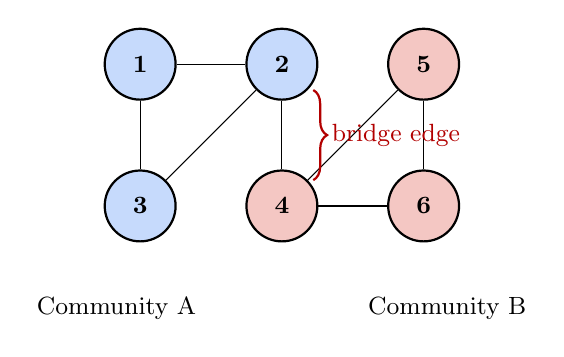
\begin{tikzpicture}[
    node distance=1.8cm,
    main/.style={circle, draw, thick, minimum size=0.9cm, font=\small\bfseries},
    every edge/.style={draw, thick}
]
    % Nodes - a small social network
    \node[main, fill=node1color!30] (1) {1};
    \node[main, fill=node1color!30, right of=1] (2) {2};
    \node[main, fill=node1color!30, below of=1] (3) {3};
    \node[main, fill=node2color!30, right of=3] (4) {4};
    \node[main, fill=node2color!30, right of=2] (5) {5};
    \node[main, fill=node2color!30, right of=4] (6) {6};
    
    % Edges
    \draw (1) -- (2);
    \draw (1) -- (3);
    \draw (2) -- (3);
    \draw (2) -- (4);
    \draw (4) -- (5);
    \draw (4) -- (6);
    \draw (5) -- (6);
    
    % Labels
    \node[below of=3, yshift=0.5cm, xshift=-0.3cm] {\small Community A};
    \node[below of=6, yshift=0.5cm, xshift=0.3cm] {\small Community B};
    
    % Bridge annotation
    \draw[decorate, decoration={brace, amplitude=5pt, raise=2pt}, thick, red!70!black] 
        (2.south east) -- (4.north east) node[midway, right, xshift=5pt, yshift=0pt, font=\small] {bridge edge};
\end{tikzpicture}
\caption{Our running example: a 6-node graph with two communities connected by a bridge edge (2--4). Nodes 1, 2, 3 form Community A; nodes 4, 5, 6 form Community B.}
\label{shallow-embeddings:fig:running_example}
\end{figure}

The adjacency matrix for this graph is:
\begin{equation}
\adj = \begin{pmatrix}
0 & 1 & 1 & 0 & 0 & 0 \\
1 & 0 & 1 & 1 & 0 & 0 \\
1 & 1 & 0 & 0 & 0 & 0 \\
0 & 1 & 0 & 0 & 1 & 1 \\
0 & 0 & 0 & 1 & 0 & 1 \\
0 & 0 & 0 & 1 & 1 & 0
\end{pmatrix}
\label{shallow-embeddings:eq:adj_matrix}
\end{equation}

\begin{intuition}
A good embedding should place nodes 1, 2, 3 close together (they're in the same community) and nodes 4, 5, 6 close together, with some distance between the two groups. Node 2 and node 4 might be somewhere in between since they're the ``bridge'' between communities.
\end{intuition}

\subsection{What Makes a Good Embedding?}

\begin{definition}[Graph Embedding]
A \textbf{graph embedding} is a mapping $\phi: V \to \R^d$ that assigns each node $v_i$ a vector $\vect{y}_i \in \R^d$. We can collect all embeddings into a matrix:
\[
\embed = \begin{pmatrix} \text{---} & \vect{y}_1^\top & \text{---} \\ \text{---} & \vect{y}_2^\top & \text{---} \\ & \vdots & \\ \text{---} & \vect{y}_n^\top & \text{---} \end{pmatrix} \in \R^{n \times d}
\]
\end{definition}

The key question is: \textbf{what does ``similar in the graph'' mean?} This leads us to different notions of proximity.

% ============================================================================
% SECTION 2: GRAPH CONCEPTS
% ============================================================================
\section{Essential Graph Concepts (With Purpose)}

We introduce each concept with its \emph{motivation}---what problem it solves or what it helps us compute.

\subsection{The Degree Matrix}

\begin{whybox}
The degree tells us how ``popular'' or ``connected'' a node is. High-degree nodes are often important hubs. We'll need the degree matrix to normalize things properly (so high-degree nodes don't dominate) and to define random walks.
\end{whybox}

\begin{definition}[Degree and Degree Matrix]
The \textbf{degree} of node $v_i$ is $d_i = \sum_{j=1}^{n} A_{ij}$ (the number of neighbors). The \textbf{degree matrix} $\degree$ is diagonal:
\[
\degree = \diag(d_1, d_2, \ldots, d_n)
\]
\end{definition}

\begin{example}
For our running example:
\[
\degree = \diag(2, 3, 2, 3, 2, 2)
\]
Node 2 and node 4 have degree 3 (they're the bridges connecting communities), while the others have degree 2.

\begin{center}
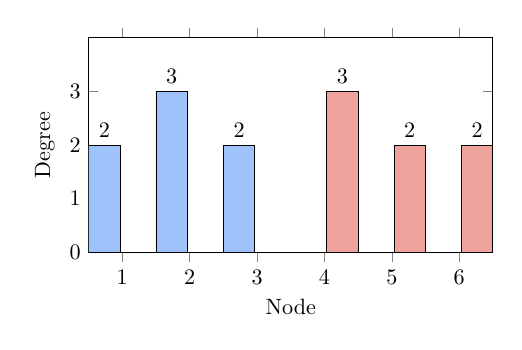
\begin{tikzpicture}[scale=0.8]
    % Bar chart of degrees
    \begin{axis}[
        ybar,
        bar width=0.5cm,
        xlabel={Node},
        ylabel={Degree},
        ymin=0, ymax=4,
        xtick={1,2,3,4,5,6},
        ytick={0,1,2,3},
        nodes near coords,
        nodes near coords align={vertical},
        width=8cm, height=5cm
    ]
    \addplot[fill=node1color!50] coordinates {(1,2) (2,3) (3,2)};
    \addplot[fill=node2color!50] coordinates {(4,3) (5,2) (6,2)};
    \end{axis}
\end{tikzpicture}
\end{center}
\end{example}

\subsection{The Graph Laplacian Family}

\begin{whybox}
The Laplacian matrices capture the ``smoothness'' of signals on graphs. They're fundamental to spectral graph theory and appear naturally when we analyze random walks, graph cuts, and clustering. Different normalizations serve different purposes.
\end{whybox}

\subsubsection*{First: What is a Signal on a Graph?}

Before introducing the Laplacian, we need to understand \textbf{graph signals}---this concept is essential for understanding what the Laplacian measures.

\begin{definition}[Graph Signal]
A \textbf{graph signal} is simply a function that assigns a value to each node:
\[
\vect{x}: V \to \R, \quad \text{i.e., } \vect{x} = (x_1, x_2, \ldots, x_n)^\top \in \R^n
\]
where $x_i$ is the value at node $v_i$.
\end{definition}

\begin{example}
On our 6-node social network, here are some example graph signals:

\begin{center}
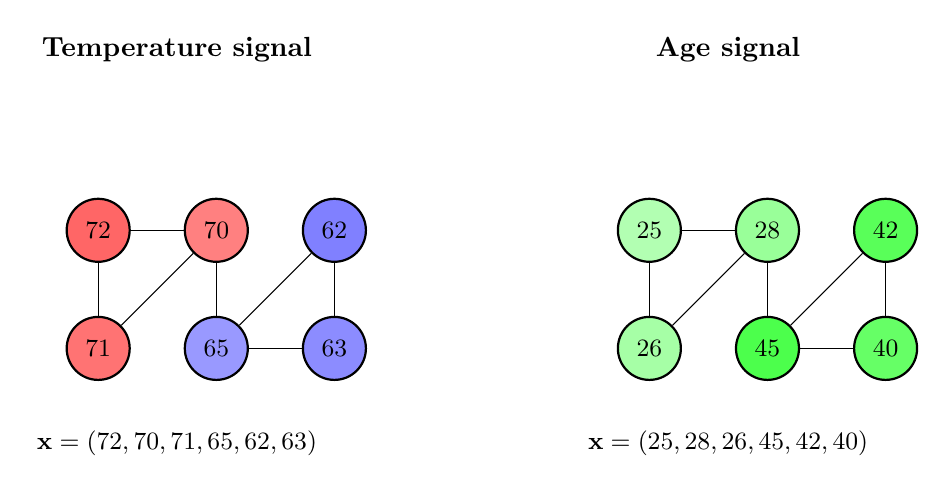
\begin{tikzpicture}[
    node distance=1.5cm,
    main/.style={circle, draw, thick, minimum size=0.8cm, font=\small},
]
    % Temperature signal
    \begin{scope}[xshift=0cm]
        \node[font=\bfseries] at (1, 2.3) {Temperature signal};
        \node[main, fill=red!60] (1) {72};
        \node[main, fill=red!50, right of=1] (2) {70};
        \node[main, fill=red!55, below of=1] (3) {71};
        \node[main, fill=blue!40, right of=3] (4) {65};
        \node[main, fill=blue!50, right of=2] (5) {62};
        \node[main, fill=blue!45, right of=4] (6) {63};
        \draw (1)--(2); \draw (1)--(3); \draw (2)--(3);
        \draw (2)--(4); \draw (4)--(5); \draw (4)--(6); \draw (5)--(6);
        \node[below of=3, yshift=0.3cm, xshift=1cm, font=\small] {$\vect{x} = (72, 70, 71, 65, 62, 63)$};
    \end{scope}
    
    % Age signal
    \begin{scope}[xshift=7cm]
        \node[font=\bfseries] at (1, 2.3) {Age signal};
        \node[main, fill=green!30] (1b) {25};
        \node[main, fill=green!40, right of=1b] (2b) {28};
        \node[main, fill=green!35, below of=1b] (3b) {26};
        \node[main, fill=green!70, right of=3b] (4b) {45};
        \node[main, fill=green!65, right of=2b] (5b) {42};
        \node[main, fill=green!60, right of=4b] (6b) {40};
        \draw (1b)--(2b); \draw (1b)--(3b); \draw (2b)--(3b);
        \draw (2b)--(4b); \draw (4b)--(5b); \draw (4b)--(6b); \draw (5b)--(6b);
        \node[below of=3b, yshift=0.3cm, xshift=1cm, font=\small] {$\vect{x} = (25, 28, 26, 45, 42, 40)$};
    \end{scope}
\end{tikzpicture}
\end{center}

\textbf{Key observation}: In many real graphs, connected nodes tend to have \emph{similar} signal values. Friends often have similar ages, neighboring sensors measure similar temperatures, etc. This property is called \textbf{smoothness}---the signal doesn't change abruptly across edges.
\end{example}

\begin{intuition}
Graph signals are everywhere:
\begin{itemize}
    \item \textbf{Social network}: Each person's age, income, or political leaning
    \item \textbf{Sensor network}: Temperature, humidity at each sensor location
    \item \textbf{Citation network}: Number of citations for each paper
    \item \textbf{Brain network}: Neural activity at each brain region
\end{itemize}
The Laplacian will help us measure how ``smooth'' a signal is---i.e., how much it varies across edges.
\end{intuition}

Now we can define the Laplacian and understand what it measures:

\begin{definition}[Graph Laplacians]
\leavevmode
\begin{itemize}
    \item The \textbf{combinatorial Laplacian}: $\lamark = \degree - \adj$
    \item The \textbf{normalized Laplacian}: $\lamark_{\text{norm}} = 
    \identity - \degree^{-1/2} \adj \degree^{-1/2}$
    \item The \textbf{random walk Laplacian}: $\lamark_{\text{rw}} = \identity - \degree^{-1} \adj$
\end{itemize}
\end{definition}

Let's see what each one does and why we need three versions:

\begin{example}
For our running example, the combinatorial Laplacian is:
\[
\lamark = \degree - \adj = \begin{pmatrix}
2 & -1 & -1 & 0 & 0 & 0 \\
-1 & 3 & -1 & -1 & 0 & 0 \\
-1 & -1 & 2 & 0 & 0 & 0 \\
0 & -1 & 0 & 3 & -1 & -1 \\
0 & 0 & 0 & -1 & 2 & -1 \\
0 & 0 & 0 & -1 & -1 & 2
\end{pmatrix}
\]

\textbf{What does the Laplacian measure?} It measures the \textbf{smoothness} (or roughness) of a signal through a beautiful formula:
\[
\vect{x}^\top \lamark \vect{x} = \sum_{(i,j) \in E} (x_i - x_j)^2
\]

\begin{mathbox}
\textbf{Proof of the Laplacian quadratic form.}

We want to compute $\vect{x}^\top \lamark \vect{x}$ where $\lamark = \degree - \adj$.

\textbf{Step 1:} Expand using linearity:
\[
\vect{x}^\top \lamark \vect{x} = \vect{x}^\top (\degree - \adj) \vect{x} = \vect{x}^\top \degree \vect{x} - \vect{x}^\top \adj \vect{x}
\]

\textbf{Step 2:} Compute the first term. Since $\degree$ is diagonal with $D_{ii} = d_i$:
\[
\vect{x}^\top \degree \vect{x} = \sum_{i=1}^{n} d_i x_i^2
\]

\textbf{Step 3:} Compute the second term:
\[
\vect{x}^\top \adj \vect{x} = \sum_{i=1}^{n} \sum_{j=1}^{n} A_{ij} x_i x_j = \sum_{(i,j) \in E} x_i x_j + \sum_{(j,i) \in E} x_j x_i = 2\sum_{(i,j) \in E} x_i x_j
\]
(The last equality holds for undirected graphs where each edge is counted twice.)

\textbf{Step 4:} Recall that $d_i = \sum_j A_{ij}$, so:
\[
\sum_{i=1}^{n} d_i x_i^2 = \sum_{i=1}^{n} \sum_{j: (i,j) \in E} x_i^2 = \sum_{(i,j) \in E} x_i^2 + \sum_{(i,j) \in E} x_j^2 = \sum_{(i,j) \in E} (x_i^2 + x_j^2)
\]
(Again, each edge contributes $x_i^2$ from node $i$'s degree and $x_j^2$ from node $j$'s degree.)

\textbf{Step 5:} Combine:
\begin{align*}
\vect{x}^\top \lamark \vect{x} &= \sum_{(i,j) \in E} (x_i^2 + x_j^2) - 2\sum_{(i,j) \in E} x_i x_j \\
&= \sum_{(i,j) \in E} (x_i^2 - 2x_i x_j + x_j^2) \\
&= \sum_{(i,j) \in E} (x_i - x_j)^2 \quad \blacksquare
\end{align*}
\end{mathbox}

This formula tells us: the Laplacian quadratic form sums up the squared differences across all edges. It is small when connected nodes have similar values, and large when they differ.

\textbf{Let's compare two signals on our graph:}

\textit{Signal 1 (smooth):} $\vect{x}_{\text{smooth}} = (1, 1, 1, 0, 0, 0)$ --- Community A has value 1, Community B has value 0.
\begin{align*}
\vect{x}_{\text{smooth}}^\top \lamark \vect{x}_{\text{smooth}} &= (1-1)^2 + (1-1)^2 + (1-1)^2 + (1-0)^2 + (0-0)^2 + (0-0)^2 + (0-0)^2 \\
&= 0 + 0 + 0 + 1 + 0 + 0 + 0 = \mathbf{1}
\end{align*}
Only the bridge edge (2--4) contributes because it connects different values!

\textit{Signal 2 (rough):} $\vect{x}_{\text{rough}} = (1, 0, 1, 0, 1, 0)$ --- Alternating pattern.
\begin{align*}
\vect{x}_{\text{rough}}^\top \lamark \vect{x}_{\text{rough}} &= (1-0)^2 + (1-1)^2 + (0-1)^2 + (0-0)^2 + (0-1)^2 + (0-0)^2 + (1-0)^2 \\
&= 1 + 0 + 1 + 0 + 1 + 0 + 1 = \mathbf{4}
\end{align*}

\begin{center}
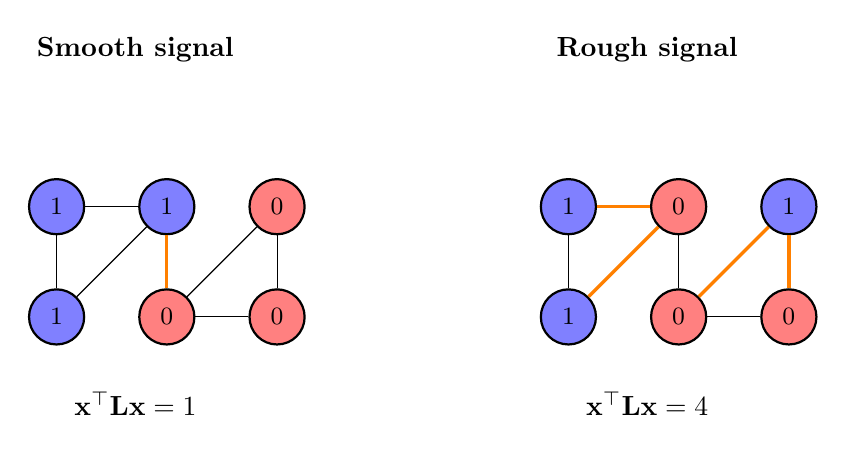
\begin{tikzpicture}[
    node distance=1.4cm,
    main/.style={circle, draw, thick, minimum size=0.7cm, font=\small},
]
    % Smooth signal
    \begin{scope}[xshift=0cm]
        \node[font=\bfseries] at (1, 2) {Smooth signal};
        \node[main, fill=blue!50] (1) {1};
        \node[main, fill=blue!50, right of=1] (2) {1};
        \node[main, fill=blue!50, below of=1] (3) {1};
        \node[main, fill=red!50, right of=3] (4) {0};
        \node[main, fill=red!50, right of=2] (5) {0};
        \node[main, fill=red!50, right of=4] (6) {0};
        \draw (1)--(2); \draw (1)--(3); \draw (2)--(3);
        \draw[very thick, orange] (2)--(4); 
        \draw (4)--(5); \draw (4)--(6); \draw (5)--(6);
        \node[below of=3, yshift=0.3cm, xshift=1cm] {$\vect{x}^\top \lamark \vect{x} = 1$};
    \end{scope}
    
    % Rough signal
    \begin{scope}[xshift=6.5cm]
        \node[font=\bfseries] at (1, 2) {Rough signal};
        \node[main, fill=blue!50] (1b) {1};
        \node[main, fill=red!50, right of=1b] (2b) {0};
        \node[main, fill=blue!50, below of=1b] (3b) {1};
        \node[main, fill=red!50, right of=3b] (4b) {0};
        \node[main, fill=blue!50, right of=2b] (5b) {1};
        \node[main, fill=red!50, right of=4b] (6b) {0};
        \draw[very thick, orange] (1b)--(2b); 
        \draw (1b)--(3b); 
        \draw[very thick, orange] (2b)--(3b);
        \draw (2b)--(4b); 
        \draw[very thick, orange] (4b)--(5b); 
        \draw (4b)--(6b); 
        \draw[very thick, orange] (5b)--(6b);
        \node[below of=3b, yshift=0.3cm, xshift=1cm] {$\vect{x}^\top \lamark \vect{x} = 4$};
    \end{scope}
\end{tikzpicture}
\end{center}

The smooth signal respects the community structure (similar values within communities), while the rough signal changes value across many edges (shown in orange).
\end{example}

\begin{keyinsight}
\textbf{Why does this matter for embeddings?} 

If we think of each dimension of an embedding as a graph signal, then a \textbf{good embedding should be smooth}---nodes that are connected should have similar embedding coordinates. 

This is exactly what matrix factorization methods optimize! When we minimize $\sum_{(i,j) \in E}(A_{ij} - \vect{y}_i^\top \vect{y}_j)^2$, we're encouraging connected nodes ($A_{ij} = 1$) to have high inner product, which means similar embeddings.
\end{keyinsight}

\begin{keyinsight}
\textbf{Why three Laplacians?} Each normalization serves a purpose:
\begin{itemize}
    \item \textbf{Combinatorial} $\lamark$: Used in spectral clustering; eigenvalues relate to graph cuts
    \item \textbf{Normalized} $\lamark_{\text{norm}}$: Eigenvalues in $[0, 2]$; better for comparing graphs of different sizes
    \item \textbf{Random walk} $\lamark_{\text{rw}}$: Directly connected to random walks; we'll use this for DeepWalk!
\end{itemize}
\end{keyinsight}

% -------------------------------------------------------------------------
% NORMALIZED LAPLACIAN - Detailed explanation
% -------------------------------------------------------------------------
\subsubsection*{The Normalized Laplacian: Fixing the Degree Bias}

\begin{whybox}
The combinatorial Laplacian has a problem: \textbf{high-degree nodes dominate the quadratic form}. If node $i$ has degree 100 and node $j$ has degree 2, differences involving node $i$ contribute much more to $\vect{x}^\top \lamark \vect{x}$. This makes it hard to compare graphs of different sizes or densities.
\end{whybox}

The normalized Laplacian fixes this by scaling each node's contribution by its degree:
\[
\lamark_{\text{norm}} = \identity - \degree^{-1/2} \adj \degree^{-1/2}
\]

\begin{mathbox}
\textbf{What does the normalized Laplacian measure?}

The quadratic form becomes:
\[
\vect{x}^\top \lamark_{\text{norm}} \vect{x} = \sum_{(i,j) \in E} \left( \frac{x_i}{\sqrt{d_i}} - \frac{x_j}{\sqrt{d_j}} \right)^2
\]

\textbf{Proof:} Let $\vect{z} = \degree^{1/2} \vect{x}$, i.e., $z_i = \sqrt{d_i} \, x_i$. Then:
\begin{align*}
\vect{x}^\top \lamark_{\text{norm}} \vect{x} &= \vect{x}^\top (\identity - \degree^{-1/2} \adj \degree^{-1/2}) \vect{x} \\
&= \vect{x}^\top \degree^{-1/2} (\degree - \adj) \degree^{-1/2} \vect{x} \\
&= (\degree^{-1/2}\vect{x})^\top \lamark (\degree^{-1/2}\vect{x})
\end{align*}

Using our earlier result with $\tilde{\vect{x}} = \degree^{-1/2}\vect{x}$ (so $\tilde{x}_i = x_i / \sqrt{d_i}$):
\[
\vect{x}^\top \lamark_{\text{norm}} \vect{x} = \sum_{(i,j) \in E} (\tilde{x}_i - \tilde{x}_j)^2 = \sum_{(i,j) \in E} \left( \frac{x_i}{\sqrt{d_i}} - \frac{x_j}{\sqrt{d_j}} \right)^2 \quad \blacksquare
\]
\end{mathbox}

\begin{example}
Consider an edge between a ``celebrity'' node (degree 100) and a ``regular'' node (degree 3):
\begin{itemize}
    \item \textbf{Combinatorial}: The difference $(x_{\text{celebrity}} - x_{\text{regular}})^2$ is treated the same as any other edge.
    \item \textbf{Normalized}: The difference becomes $\left( \frac{x_{\text{celebrity}}}{10} - \frac{x_{\text{regular}}}{\sqrt{3}} \right)^2$. The celebrity's value is scaled down by $\sqrt{100} = 10$, reducing its outsized influence.
\end{itemize}

\textbf{Key property}: The normalized Laplacian has eigenvalues in $[0, 2]$ regardless of graph size. This makes it ideal for:
\begin{itemize}
    \item Comparing spectral properties across different graphs
    \item Spectral clustering (the famous ``normalized cuts'' algorithm)
    \item Theoretical analysis (bounded spectrum simplifies proofs)
\end{itemize}
\end{example}

% -------------------------------------------------------------------------
% RANDOM WALK LAPLACIAN - Why define it?
% -------------------------------------------------------------------------
\subsubsection*{The Random Walk Laplacian: More Than Just $\identity - \transition$}

\begin{whybox}
You might wonder: if all we need for DeepWalk is the transition matrix $\transition = \degree^{-1}\adj$, why bother defining the random walk Laplacian $\lamark_{\text{rw}} = \identity - \transition$? The answer is that $\lamark_{\text{rw}}$ reveals a \textbf{deep connection between random walks and graph smoothness}.
\end{whybox}

\begin{mathbox}
\textbf{The random walk Laplacian quadratic form:}
\[
\vect{x}^\top \lamark_{\text{rw}} \vect{x} = \sum_{(i,j) \in E} \frac{1}{d_i}(x_i - x_j)^2
\]

This is an \textbf{asymmetric} version of smoothness: differences are weighted by $1/d_i$, not $1/\sqrt{d_i d_j}$.

\textbf{Interpretation}: This measures smoothness from the perspective of a random walker. A walker at node $i$ sees each neighbor with probability $1/d_i$, so edges from high-degree nodes contribute less.
\end{mathbox}

The key insight is the \textbf{relationship between all three Laplacians}:

\begin{proposition}[Similarity of Laplacians]
The three Laplacians share the same eigenvalues structure:
\begin{itemize}
    \item $\lamark_{\text{rw}}$ and $\lamark_{\text{norm}}$ have \textbf{exactly the same eigenvalues}
    \item If $\vect{v}$ is an eigenvector of $\lamark_{\text{norm}}$ with eigenvalue $\lambda$, then $\degree^{-1/2}\vect{v}$ is an eigenvector of $\lamark_{\text{rw}}$ with the same eigenvalue $\lambda$
\end{itemize}
\end{proposition}

\begin{proof}
If $\lamark_{\text{norm}} \vect{v} = \lambda \vect{v}$, then:
\begin{align*}
(\identity - \degree^{-1/2}\adj\degree^{-1/2})\vect{v} &= \lambda \vect{v} \\
\degree^{-1/2}(\identity - \degree^{-1/2}\adj\degree^{-1/2})\vect{v} &= \lambda \degree^{-1/2}\vect{v} \\
(\degree^{-1/2} - \degree^{-1}\adj\degree^{-1/2})\vect{v} &= \lambda \degree^{-1/2}\vect{v} \\
(\identity - \degree^{-1}\adj)\degree^{-1/2}\vect{v} &= \lambda \degree^{-1/2}\vect{v} \\
\lamark_{\text{rw}} (\degree^{-1/2}\vect{v}) &= \lambda (\degree^{-1/2}\vect{v}) \quad \blacksquare
\end{align*}
\end{proof}

\begin{keyinsight}
\textbf{Why does this matter?}

This connection explains why DeepWalk (which uses random walks, i.e., $\transition = \identity - \lamark_{\text{rw}}$) learns spectral information about the graph:
\begin{enumerate}
    \item Random walks sample nodes according to the transition matrix $\transition$
    \item The transition matrix is directly related to $\lamark_{\text{rw}}$
    \item $\lamark_{\text{rw}}$ shares eigenvalues with $\lamark_{\text{norm}}$
    \item Therefore, \textbf{DeepWalk implicitly learns the spectral structure} of the normalized Laplacian!
\end{enumerate}

This is formalized in the theorem we'll see later: DeepWalk embeddings approximate eigenvectors of a matrix related to $\sum_{r=1}^{c} \transition^r$.
\end{keyinsight}

\begin{example}[Random Walk Laplacian in Action]
The matrix $\transition = \degree^{-1}\adj = \identity - \lamark_{\text{rw}}$ is the \textbf{transition matrix} of a random walk:
\[
\transition = \begin{pmatrix}
0 & 1/2 & 1/2 & 0 & 0 & 0 \\
1/3 & 0 & 1/3 & 1/3 & 0 & 0 \\
1/2 & 1/2 & 0 & 0 & 0 & 0 \\
0 & 1/3 & 0 & 0 & 1/3 & 1/3 \\
0 & 0 & 0 & 1/2 & 0 & 1/2 \\
0 & 0 & 0 & 1/2 & 1/2 & 0
\end{pmatrix}
\]

Entry $P_{ij}$ is the probability of jumping from node $i$ to node $j$. From node 2, we go to nodes 1, 3, or 4 each with probability $1/3$.

\textbf{This is exactly what DeepWalk uses!} Random walks on graphs generate ``sentences'' of nodes, which we then feed to a skip-gram model.
\end{example}

\begin{table}[htbp]
\centering
\caption{Summary: The Three Laplacians}
\begin{tabular}{@{}lccc@{}}
\toprule
\textbf{Laplacian} & \textbf{Formula} & \textbf{Quadratic Form} & \textbf{Main Use} \\
\midrule
Combinatorial & $\degree - \adj$ & $\sum_{(i,j)} (x_i - x_j)^2$ & Graph cuts, basic spectral \\
Normalized & $\identity - \degree^{-1/2}\adj\degree^{-1/2}$ & $\sum_{(i,j)} \left(\frac{x_i}{\sqrt{d_i}} - \frac{x_j}{\sqrt{d_j}}\right)^2$ & Normalized cuts, comparison \\
Random walk & $\identity - \degree^{-1}\adj$ & $\sum_{(i,j)} \frac{1}{d_i}(x_i - x_j)^2$ & Random walks, DeepWalk \\
\bottomrule
\end{tabular}
\label{shallow-embeddings:tab:laplacians}
\end{table}

\subsection{Notions of Proximity: How to Measure ``Similarity'' in Graphs}

Different embedding methods preserve different notions of similarity. Understanding these is crucial for choosing the right method.

\begin{definition}[First-Order Proximity]
Two nodes have high \textbf{first-order proximity} if they are directly connected:
\[
s^{(1)}_{ij} = A_{ij}
\]
\end{definition}

\begin{definition}[Second-Order Proximity]
Two nodes have high \textbf{second-order proximity} if they share many neighbors (even if not directly connected):
\[
s^{(2)}_{ij} = \text{similarity of neighborhood}(\vect{a}_i, \vect{a}_j)
\]
where $\vect{a}_i$ is the $i$-th row of $\adj$.
\end{definition}

\begin{example}
In our graph, consider nodes 1 and 4:
\begin{itemize}
    \item \textbf{First-order proximity}: $A_{14} = 0$ (not directly connected)
    \item \textbf{Second-order proximity}: Node 1's neighbors are $\{2, 3\}$. Node 4's neighbors are $\{2, 5, 6\}$. They share neighbor 2, so they have \emph{some} second-order proximity.
\end{itemize}

Now consider nodes 1 and 6:
\begin{itemize}
    \item First-order: $A_{16} = 0$
    \item Second-order: Node 1's neighbors $\{2,3\}$ vs node 6's neighbors $\{4,5\}$---no overlap! Very low second-order proximity.
\end{itemize}

\textbf{Conclusion}: Even though both (1,4) and (1,6) are not directly connected, nodes 1 and 4 are ``more similar'' in the second-order sense.
\end{example}

\begin{figure}[htbp]
\centering
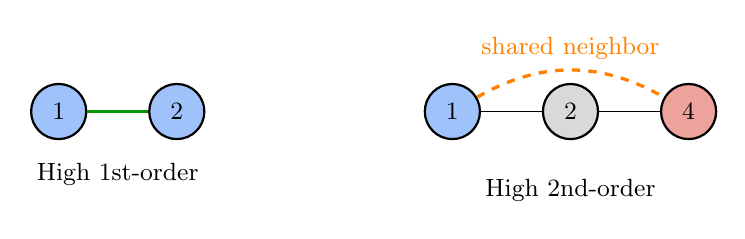
\begin{tikzpicture}[
    node distance=1.5cm,
    main/.style={circle, draw, thick, minimum size=0.7cm, font=\small},
]
    % First-order example
    \begin{scope}[xshift=0cm]
        \node[main, fill=node1color!50] (a) {1};
        \node[main, fill=node1color!50, right of=a] (b) {2};
        \draw[very thick, green!60!black] (a) -- (b);
        \node[below of=a, yshift=0.7cm, xshift=0.75cm] {\small High 1st-order};
    \end{scope}
    
    % Second-order example
    \begin{scope}[xshift=5cm]
        \node[main, fill=node1color!50] (c) {1};
        \node[main, fill=gray!30, right of=c] (d) {2};
        \node[main, fill=node2color!50, right of=d] (e) {4};
        \draw (c) -- (d);
        \draw (d) -- (e);
        \draw[dashed, orange, very thick] (c) to[bend left=30] node[above, font=\small] {shared neighbor} (e);
        \node[below of=d, yshift=0.5cm] {\small High 2nd-order};
    \end{scope}
\end{tikzpicture}
\caption{First-order proximity (direct edge) vs second-order proximity (shared neighbors).}
\label{shallow-embeddings:fig:proximity_types}
\end{figure}

\begin{definition}[$k$-th Order Proximity]
The \textbf{$k$-th order proximity} captures indirect connections through paths of length $k$:
\[
s^{(k)}_{ij} = (\adj^k)_{ij} = \text{number of paths of length } k \text{ from } i \text{ to } j
\]
\end{definition}

\begin{example}
Let's compute $\adj^2$ for our graph (paths of length 2):
\[
\adj^2 = \begin{pmatrix}
2 & 1 & 1 & 1 & 0 & 0 \\
1 & 3 & 1 & 0 & 1 & 1 \\
1 & 1 & 2 & 1 & 0 & 0 \\
1 & 0 & 1 & 3 & 1 & 1 \\
0 & 1 & 0 & 1 & 2 & 1 \\
0 & 1 & 0 & 1 & 1 & 2
\end{pmatrix}
\]

Reading off: there are 3 paths of length 2 from node 2 to itself (2→1→2, 2→3→2, 2→4→2), confirming that node 2 is well-connected.

$(\adj^2)_{14} = 1$: there's exactly one path of length 2 from node 1 to node 4 (1→2→4).
\end{example}

\begin{definition}[High-Order Proximity: Katz Index]
The \textbf{Katz index} combines all path lengths with decaying weights:
\[
\similarity_{\text{Katz}} = \sum_{k=1}^{\infty} \beta^k \adj^k = \beta\adj + \beta^2\adj^2 + \beta^3\adj^3 + \cdots
\]
where $\beta < 1/\lambda_{\max}(\adj)$ ensures convergence. This can be computed in closed form:
\[
\similarity_{\text{Katz}} = (\identity - \beta\adj)^{-1} - \identity
\]
\end{definition}

\begin{intuition}
The Katz index says: ``nodes are similar if there are many paths between them, but longer paths count less.'' The parameter $\beta$ controls how quickly long paths are discounted. With $\beta = 0.1$:
\begin{itemize}
    \item Direct neighbors (length 1): contribute $0.1$
    \item Length-2 paths: contribute $0.01$ each
    \item Length-3 paths: contribute $0.001$ each
\end{itemize}
\end{intuition}


% ============================================================================
% SECTION 3: MATRIX FACTORIZATION METHODS
% ============================================================================
\section{Matrix Factorization Methods}

The idea is beautifully simple: if we can write the adjacency (or similarity) matrix as a product of low-rank matrices, those factors give us embeddings!

\subsection{The Core Idea}

\begin{keyinsight}
If $\adj \approx \embed \embed^\top$ where $\embed \in \R^{n \times d}$, then:
\[
A_{ij} \approx \vect{y}_i^\top \vect{y}_j
\]
Connected nodes ($A_{ij} = 1$) should have $\vect{y}_i^\top \vect{y}_j \approx 1$, meaning their embeddings point in similar directions. Non-edges ($A_{ij} = 0$) should have $\vect{y}_i^\top \vect{y}_j \approx 0$, meaning orthogonal embeddings.
\end{keyinsight}

\begin{alarmbox}[The Diagonal Problem]
There's an issue with the naive interpretation ``$\adj \approx \embed\embed^\top$''! 

The diagonal entries of $\embed \embed^\top$ are:
\[
(\embed \embed^\top)_{ii} = \vect{y}_i^\top \vect{y}_i = \|\vect{y}_i\|^2
\]
But for graphs without self-loops, the diagonal of the adjacency matrix is zero: $A_{ii} = 0$. 

So a true factorization $\adj = \embed\embed^\top$ would require $\|\vect{y}_i\|^2 = 0$ for all nodes---meaning all embeddings are the zero vector! That's clearly useless.

\textbf{Solution}: We \textbf{only fit the off-diagonal entries}. The Graph Factorization loss sums over edges $(i,j) \in E$ where $i \neq j$, completely ignoring the diagonal. We're not truly factorizing $\adj$; we're finding embeddings whose inner products approximate the \emph{edge weights}.
\end{alarmbox}

\begin{figure}[htbp]
\centering
\begin{tikzpicture}
    % Matrix visualization with highlighted diagonal
    \node at (0, 0) {
        $\underbrace{\begin{pmatrix} 
        \textcolor{red}{0} & 1 & 1 & 0 & 0 & 0 \\
        1 & \textcolor{red}{0} & 1 & 1 & 0 & 0 \\
        1 & 1 & \textcolor{red}{0} & 0 & 0 & 0 \\
        0 & 1 & 0 & \textcolor{red}{0} & 1 & 1 \\
        0 & 0 & 0 & 1 & \textcolor{red}{0} & 1 \\
        0 & 0 & 0 & 1 & 1 & \textcolor{red}{0}
        \end{pmatrix}}_{\adj \in \R^{6 \times 6}}$
    };
    
    \node at (2.5, 0) {$\approx$};
    
    \node at (4.5, 0) {
        $\underbrace{\begin{pmatrix}
        \leftarrow & \vect{y}_1^\top & \rightarrow \\
        \leftarrow & \vect{y}_2^\top & \rightarrow \\
        & \vdots & \\
        \leftarrow & \vect{y}_6^\top & \rightarrow
        \end{pmatrix}}_{\embed \in \R^{6 \times d}}$
    };
    
    \node at (6.5, 0) {$\times$};
    
    \node at (7.5, 0) {$\embed^\top$};
    
    % Annotation about diagonal
    \node[below, text width=8cm, align=center, font=\small] at (3.5, -2.2) {
        The \textcolor{red}{diagonal} of $\adj$ is zero, but $(\embed\embed^\top)_{ii} = \|\vect{y}_i\|^2$.\\
        We only fit the off-diagonal entries.
    };
\end{tikzpicture}
\caption{Matrix factorization idea: we approximate the \emph{off-diagonal} entries of $\adj$ (the edges) using inner products of embedding vectors. The diagonal is ignored.}
\end{figure}

\subsection{Graph Factorization (GF)}

\begin{definition}[Graph Factorization Objective]
Find $\embed \in \R^{n \times d}$ minimizing:
\[
\mathcal{L}_{\text{GF}} = \frac{1}{2} \sum_{(i,j) \in E} \left(A_{ij} - \vect{y}_i^\top \vect{y}_j\right)^2 + \frac{\lambda}{2} \sum_{i=1}^{n} \norm{\vect{y}_i}^2
\]
\end{definition}

\begin{intuition}
\textbf{Why only sum over edges?} Two reasons:
\begin{enumerate}
    \item \textbf{Efficiency}: Only $O(m)$ terms instead of $O(n^2)$
    \item \textbf{Sparsity}: We observe edges; non-edges might be missing data, not true negatives
\end{enumerate}
The regularization $\lambda \norm{\vect{y}_i}^2$ prevents embeddings from growing too large.
\end{intuition}

\begin{example}
Let's trace through one gradient update for our graph with $d=2$ dimensions.

Suppose current embeddings are (randomly initialized):
\begin{align*}
\vect{y}_1 &= (0.5, 0.3) \\
\vect{y}_2 &= (0.4, 0.6)
\end{align*}

For edge (1,2) with $A_{12} = 1$:
\[
\text{Predicted: } \vect{y}_1^\top \vect{y}_2 = 0.5 \times 0.4 + 0.3 \times 0.6 = 0.38
\]
\[
\text{Error: } e_{12} = A_{12} - \vect{y}_1^\top \vect{y}_2 = 1 - 0.38 = 0.62
\]

The gradient update (with learning rate $\eta = 0.1$, $\lambda = 0.01$):
\begin{align*}
\vect{y}_1 &\leftarrow \vect{y}_1 + \eta(e_{12} \cdot \vect{y}_2 - \lambda \vect{y}_1) \\
&= (0.5, 0.3) + 0.1(0.62 \times (0.4, 0.6) - 0.01 \times (0.5, 0.3)) \\
&= (0.5, 0.3) + 0.1((0.248, 0.372) - (0.005, 0.003)) \\
&= (0.5, 0.3) + (0.0243, 0.0369) \\
&= (0.524, 0.337)
\end{align*}

The embedding $\vect{y}_1$ moved \emph{toward} $\vect{y}_2$ because they're connected!
\end{example}

\begin{algorithm}
\caption{Graph Factorization (Stochastic Gradient Descent)}
\begin{algorithmic}[1]
\Require Graph $G = (V, E)$, dimension $d$, learning rate $\eta$, regularization $\lambda$
\State Initialize $\vect{y}_i \sim \mathcal{N}(0, 1/d)$ for all nodes
\For{each epoch}
    \For{each edge $(i,j) \in E$ in random order}
        \State $e_{ij} \gets A_{ij} - \vect{y}_i^\top \vect{y}_j$ \Comment{reconstruction error}
        \State $\vect{y}_i \gets \vect{y}_i + \eta(e_{ij} \cdot \vect{y}_j - \lambda \vect{y}_i)$
        \State $\vect{y}_j \gets \vect{y}_j + \eta(e_{ij} \cdot \vect{y}_i - \lambda \vect{y}_j)$
    \EndFor
\EndFor
\end{algorithmic}
\end{algorithm}

\begin{figure}[htbp]
\centering
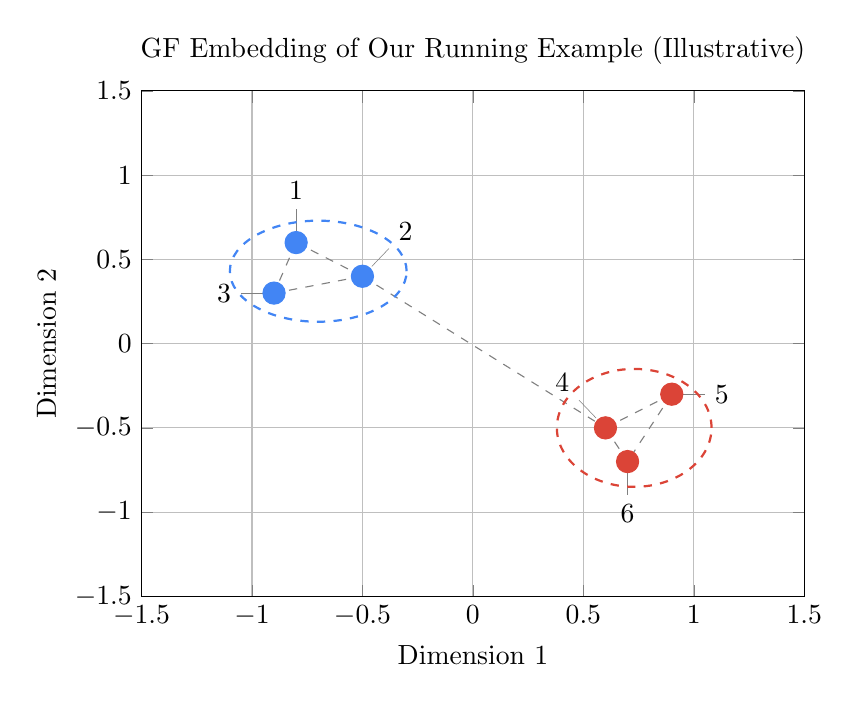
\begin{tikzpicture}
    \begin{axis}[
        width=10cm, height=8cm,
        xlabel={Dimension 1},
        ylabel={Dimension 2},
        xmin=-1.5, xmax=1.5,
        ymin=-1.5, ymax=1.5,
        grid=both,
        title={GF Embedding of Our Running Example (Illustrative)}
    ]
    % Community A - clustered together
    \addplot[only marks, mark=*, mark size=4pt, color=node1color] 
        coordinates {(-0.8, 0.6) (-0.5, 0.4) (-0.9, 0.3)};
    \node[pin={[pin distance=0.3cm]90:{1}}] at (axis cs:-0.8,0.6) {};
    \node[pin={[pin distance=0.3cm]45:{2}}] at (axis cs:-0.5,0.4) {};
    \node[pin={[pin distance=0.3cm]180:{3}}] at (axis cs:-0.9,0.3) {};
    
    % Community B - clustered together  
    \addplot[only marks, mark=*, mark size=4pt, color=node2color]
        coordinates {(0.6, -0.5) (0.9, -0.3) (0.7, -0.7)};
    \node[pin={[pin distance=0.3cm]135:{4}}] at (axis cs:0.6,-0.5) {};
    \node[pin={[pin distance=0.3cm]0:{5}}] at (axis cs:0.9,-0.3) {};
    \node[pin={[pin distance=0.3cm]-90:{6}}] at (axis cs:0.7,-0.7) {};
    
    % Draw edges as light lines
    \draw[gray, thin, dashed] (axis cs:-0.8,0.6) -- (axis cs:-0.5,0.4);
    \draw[gray, thin, dashed] (axis cs:-0.8,0.6) -- (axis cs:-0.9,0.3);
    \draw[gray, thin, dashed] (axis cs:-0.5,0.4) -- (axis cs:-0.9,0.3);
    \draw[gray, thin, dashed] (axis cs:-0.5,0.4) -- (axis cs:0.6,-0.5);
    \draw[gray, thin, dashed] (axis cs:0.6,-0.5) -- (axis cs:0.9,-0.3);
    \draw[gray, thin, dashed] (axis cs:0.6,-0.5) -- (axis cs:0.7,-0.7);
    \draw[gray, thin, dashed] (axis cs:0.9,-0.3) -- (axis cs:0.7,-0.7);
    
    % Ellipses around communities
    \draw[node1color, thick, dashed] (axis cs:-0.7,0.43) ellipse [x radius=0.4, y radius=0.3];
    \draw[node2color, thick, dashed] (axis cs:0.73,-0.5) ellipse [x radius=0.35, y radius=0.35];
    
    \end{axis}
\end{tikzpicture}
\caption{Illustrative GF embedding: nodes within the same community cluster together; the two communities are separated in embedding space.}
\label{shallow-embeddings:fig:gf_embedding}
\end{figure}

\textbf{Limitations of GF}:
\begin{itemize}
    \item Only uses first-order proximity (direct edges)
    \item Ignores non-edges completely (might miss structural information)
    \item Symmetric: can't handle directed graphs naturally
\end{itemize}

\subsection{HOPE: High-Order Proximity Preserved Embedding}

\begin{whybox}
GF only looks at direct neighbors. But in many applications, we care about broader context: ``these two people aren't friends, but they have many mutual friends.'' HOPE captures this by factorizing a \emph{high-order similarity matrix} instead of just $\adj$.
\end{whybox}

\begin{definition}[HOPE Objective]
Given a high-order proximity matrix $\similarity$ (e.g., Katz index), find \textbf{source} embeddings $\embed_s$ and \textbf{target} embeddings $\embed_t$ minimizing:
\[
\mathcal{L}_{\text{HOPE}} = \frobnorm{\similarity - \embed_s \embed_t^\top}^2
\]
\end{definition}

\begin{keyinsight}
\textbf{Why two embedding matrices?} For directed graphs, ``node $i$ influences node $j$'' is different from ``node $j$ influences node $i$.'' Having separate source and target embeddings captures this asymmetry:
\[
S_{ij} \approx \vect{y}_{s,i}^\top \vect{y}_{t,j} \neq \vect{y}_{s,j}^\top \vect{y}_{t,i} \approx S_{ji}
\]
For undirected graphs, you can use $\embed_s = \embed_t$.
\end{keyinsight}

\begin{example}
Let's compute the Katz similarity for our graph with $\beta = 0.1$:
\[
\similarity_{\text{Katz}} = (\identity - 0.1 \cdot \adj)^{-1} - \identity
\]

After computation (using a calculator or computer):
\[
\similarity_{\text{Katz}} \approx \begin{pmatrix}
0.06 & 0.14 & 0.14 & 0.05 & 0.02 & 0.02 \\
0.14 & 0.10 & 0.14 & 0.14 & 0.05 & 0.05 \\
0.14 & 0.14 & 0.06 & 0.05 & 0.02 & 0.02 \\
0.05 & 0.14 & 0.05 & 0.10 & 0.14 & 0.14 \\
0.02 & 0.05 & 0.02 & 0.14 & 0.06 & 0.14 \\
0.02 & 0.05 & 0.02 & 0.14 & 0.14 & 0.06
\end{pmatrix}
\]

Notice:
\begin{itemize}
    \item $S_{12} = S_{23} = 0.14$ (directly connected nodes have high similarity)
    \item $S_{14} = 0.05$ (not connected, but reachable via node 2)
    \item $S_{16} = 0.02$ (far apart in the graph---low similarity)
    \item $S_{24} = 0.14$ (the bridge edge creates strong similarity)
\end{itemize}

HOPE would factorize this matrix, producing embeddings where these similarities are preserved.
\end{example}

\textbf{Solution via SVD}: The optimal solution uses the Singular Value Decomposition:
\[
\similarity \approx \mathbf{U}_d \mathbf{\Sigma}_d \mathbf{V}_d^\top
\]
Setting $\embed_s = \mathbf{U}_d \mathbf{\Sigma}_d^{1/2}$ and $\embed_t = \mathbf{V}_d \mathbf{\Sigma}_d^{1/2}$ gives the best rank-$d$ approximation.

\subsection{GraRep: Multi-Scale Proximity}

\begin{whybox}
Different applications need different scales of information. Community detection needs global structure; link prediction needs local structure.
GraRep learns \emph{separate embeddings for each scale} and concatenates them.
\end{whybox}

\begin{definition}[GraRep]
For each $k \in \{1, 2, \ldots, K\}$, GraRep:
\begin{enumerate}
    \item Computes the $k$-step transition probability matrix $\transition^k$
    \item Applies a log-transformation to get $\mathbf{X}^{(k)}$
    \item Factorizes $\mathbf{X}^{(k)}$ via SVD to get $d$-dimensional embeddings $\embed^{(k)} \in \R^{n \times d}$
\end{enumerate}
Final embedding: $\vect{y}_i = [\vect{y}_i^{(1)} | \vect{y}_i^{(2)} | \cdots | \vect{y}_i^{(K)}] \in \R^{Kd}$
\end{definition}

\subsubsection*{The Log-Transformation: Why and What?}

\begin{whybox}
Why not just factorize $\transition^k$ directly? The issue is that transition probabilities are \textbf{not the right quantity to preserve}. GraRep draws inspiration from word2vec's skip-gram, which implicitly factorizes a \textbf{Pointwise Mutual Information (PMI)} matrix, not raw co-occurrence counts.
\end{whybox}

The log-transformation converts transition probabilities into PMI-like quantities:

\begin{definition}[GraRep's Log-Transformation]
For the $k$-step transition matrix $\transition^k$, define:
\[
X^{(k)}_{ij} = \max\left( \log\left( \frac{(\transition^k)_{ij}}{\sum_{\ell} (\transition^k)_{\ell j}} \right) - \log(1/n), \; 0 \right)
\]
Or more simply, using the column-normalized matrix $\tilde{\transition}^k$ where each column sums to 1:
\[
X^{(k)}_{ij} = \max\left( \log(n \cdot \tilde{P}^{(k)}_{ij}), \; 0 \right)
\]
\end{definition}

\begin{intuition}
\textbf{What does this formula mean?}

\begin{itemize}
    \item $(\transition^k)_{ij}$ is the probability of reaching $j$ from $i$ in $k$ steps
    \item The denominator $\sum_{\ell} (\transition^k)_{\ell j}$ measures how ``popular'' node $j$ is as a destination
    \item The ratio $\frac{(\transition^k)_{ij}}{\sum_{\ell} (\transition^k)_{\ell j}}$ asks: ``Is node $i$ \emph{unexpectedly} likely to reach $j$, compared to random?''
    \item Taking $\log$ converts multiplicative relationships to additive (easier to factorize)
    \item The $\max(\cdot, 0)$ clips negative values (like Positive PMI in NLP)
\end{itemize}

\textbf{Why is this better?} Raw probabilities favor high-degree nodes (everyone can reach popular nodes). The log-ratio corrects for this, emphasizing \emph{specific} relationships over generic popularity.
\end{intuition}

\begin{example}
Consider nodes 1 and 4 in our graph at $k=2$:
\begin{itemize}
    \item $(\transition^2)_{14} = 0.17$ (probability of going from 1 to 4 in 2 steps)
    \item Node 4 is reachable from many nodes, so $\sum_{\ell} (\transition^2)_{\ell 4}$ is relatively large
    \item The log-ratio will be moderate: node 1 can reach node 4, but so can others
\end{itemize}

Compare to nodes 1 and 3:
\begin{itemize}
    \item $(\transition^2)_{13} = 0.17$ (same raw probability!)
    \item But node 3 is only easily reachable from the small community A
    \item The log-ratio will be higher: node 1 has a \emph{specific} relationship to node 3
\end{itemize}
\end{example}

\subsubsection*{The Concatenation: It's a Big Vector!}

\begin{keyinsight}
If we use:
\begin{itemize}
    \item $K$ scales (e.g., $K = 4$ for 1-hop, 2-hop, 3-hop, 4-hop)
    \item $d$ dimensions per scale (e.g., $d = 64$)
\end{itemize}
Then each node's final embedding has dimension $K \times d = 4 \times 64 = 256$.

\textbf{This is by design}: each scale captures different information, and we want to preserve all of it. The downstream ML algorithm can learn which scales matter for the specific task.
\end{keyinsight}

\begin{figure}[htbp]
\centering
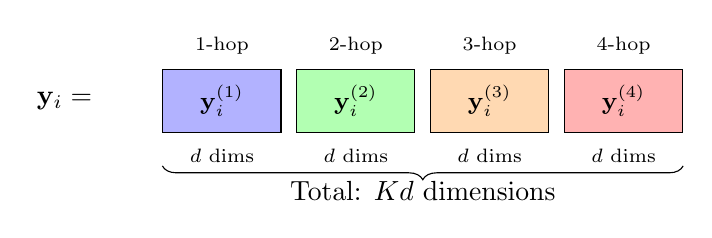
\begin{tikzpicture}[
    box/.style={rectangle, draw, minimum width=1.5cm, minimum height=0.8cm, font=\small},
    arrow/.style={-{Stealth}, thick}
]
    % Node label
    \node at (-1.5, 0) {$\vect{y}_i =$};
    
    % Embedding boxes
    \node[box, fill=blue!30] (e1) at (0.5, 0) {$\vect{y}_i^{(1)}$};
    \node[box, fill=green!30] (e2) at (2.2, 0) {$\vect{y}_i^{(2)}$};
    \node[box, fill=orange!30] (e3) at (3.9, 0) {$\vect{y}_i^{(3)}$};
    \node[box, fill=red!30] (e4) at (5.6, 0) {$\vect{y}_i^{(4)}$};
    
    % Dimension labels
    \node[below of=e1, yshift=0.3cm, font=\scriptsize] {$d$ dims};
    \node[below of=e2, yshift=0.3cm, font=\scriptsize] {$d$ dims};
    \node[below of=e3, yshift=0.3cm, font=\scriptsize] {$d$ dims};
    \node[below of=e4, yshift=0.3cm, font=\scriptsize] {$d$ dims};
    
    % Scale labels
    \node[above of=e1, yshift=-0.3cm, font=\scriptsize] {1-hop};
    \node[above of=e2, yshift=-0.3cm, font=\scriptsize] {2-hop};
    \node[above of=e3, yshift=-0.3cm, font=\scriptsize] {3-hop};
    \node[above of=e4, yshift=-0.3cm, font=\scriptsize] {4-hop};
    
    % Brace
    \draw[decorate, decoration={brace, amplitude=5pt, raise=12pt}] 
        (e4.south east) -- (e1.south west) node[midway, above, yshift=-28pt] {Total: $Kd$ dimensions};
\end{tikzpicture}
\caption{GraRep concatenates embeddings from each scale $k$. With $K=4$ scales and $d=64$ dimensions each, the final embedding has $256$ dimensions.}
\label{shallow-embeddings:fig:grarep_concat}
\end{figure}

\begin{remark}[Practical Considerations]
\leavevmode
\begin{itemize}
    \item \textbf{Choosing $K$}: Typically $K \in \{3, 4, 5\}$. Beyond $k \approx 5$, random walks mix and all nodes look similar (approach stationary distribution).
    \item \textbf{Choosing $d$}: Often $d \in \{32, 64\}$ per scale. Total dimension $Kd$ should balance expressiveness vs.\ overfitting.
    \item \textbf{Computational cost}: Computing $\transition^k$ for large $k$ is expensive ($O(n^2)$ per matrix multiplication). In practice, sparse approximations are used.
    \item \textbf{Alternative}: Instead of concatenation, some variants \emph{weight} the scales differently or learn the weights.
\end{itemize}
\end{remark}

\begin{example}
For our graph, let's see what different values of $k$ capture.

\textbf{$k=1$ (direct neighbors)}:
\[
\transition^1 = \degree^{-1}\adj = \begin{pmatrix}
0 & 0.5 & 0.5 & 0 & 0 & 0 \\
0.33 & 0 & 0.33 & 0.33 & 0 & 0 \\
0.5 & 0.5 & 0 & 0 & 0 & 0 \\
0 & 0.33 & 0 & 0 & 0.33 & 0.33 \\
0 & 0 & 0 & 0.5 & 0 & 0.5 \\
0 & 0 & 0 & 0.5 & 0.5 & 0
\end{pmatrix}
\]

\textbf{$k=2$ (two-hop neighbors)}:
\[
\transition^2 \approx \begin{pmatrix}
0.42 & 0.25 & 0.17 & 0.17 & 0 & 0 \\
0.17 & 0.39 & 0.17 & 0 & 0.11 & 0.11 \\
0.17 & 0.25 & 0.42 & 0.17 & 0 & 0 \\
0.11 & 0 & 0.11 & 0.39 & 0.17 & 0.17 \\
0 & 0.17 & 0 & 0.17 & 0.42 & 0.25 \\
0 & 0.17 & 0 & 0.17 & 0.25 & 0.42
\end{pmatrix}
\]

Notice: at $k=2$, node 1 now has non-zero ``similarity'' to node 4 (via node 2), but zero to nodes 5 and 6 (too far away).

\textbf{$k=3$ (three-hop)}:
\[
(\transition^3)_{15} > 0 \text{ and } (\transition^3)_{16} > 0
\]
Now even nodes 1 and 5/6 are connected through paths!

\begin{center}
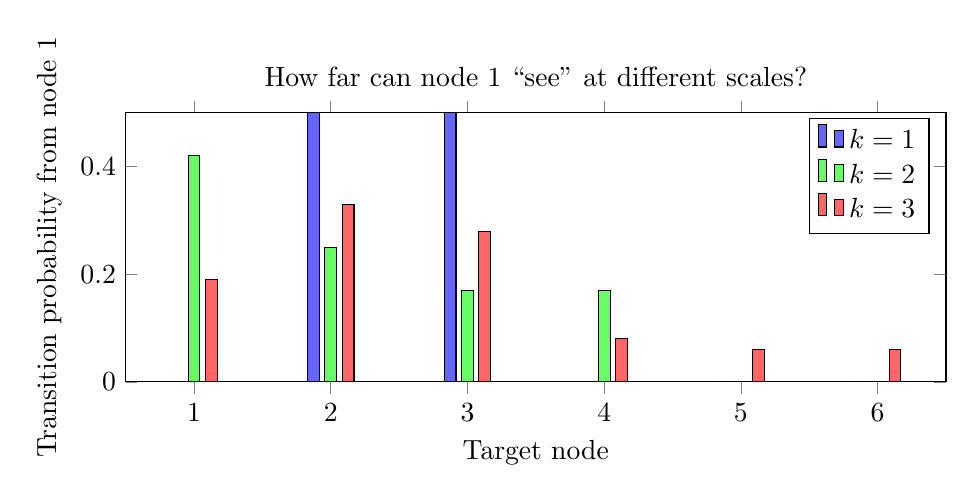
\begin{tikzpicture}
    \begin{axis}[
        width=12cm, height=5cm,
        ybar,
        bar width=0.15cm,
        xlabel={Target node},
        ylabel={Transition probability from node 1},
        ymin=0, ymax=0.5,
        xtick={1,2,3,4,5,6},
        legend style={at={(0.98,0.98)}, anchor=north east},
        title={How far can node 1 ``see'' at different scales?}
    ]
    \addplot[fill=blue!60] coordinates {(1,0) (2,0.5) (3,0.5) (4,0) (5,0) (6,0)};
    \addplot[fill=green!60] coordinates {(1,0.42) (2,0.25) (3,0.17) (4,0.17) (5,0) (6,0)};
    \addplot[fill=red!60] coordinates {(1,0.19) (2,0.33) (3,0.28) (4,0.08) (5,0.06) (6,0.06)};
    \legend{$k=1$, $k=2$, $k=3$}
    \end{axis}
\end{tikzpicture}
\end{center}
\end{example}

\begin{keyinsight}
GraRep's multi-scale approach is powerful because:
\begin{itemize}
    \item Small $k$: captures local structure (who are my immediate friends?)
    \item Large $k$: captures global structure (what community am I in?)
\end{itemize}
By concatenating embeddings from all scales, we get the best of both worlds.
\end{keyinsight}


% ============================================================================
% SECTION 4: SKIP-GRAM METHODS
% ============================================================================
\section{Skip-Gram Based Methods}

These methods borrow a brilliant idea from natural language processing: \emph{you can learn word meanings from context}. The same idea applies to graphs!

\subsection{From Words to Nodes: The Key Insight}

\begin{intuition}
In a sentence, nearby words are related: ``The \underline{cat} sat on the \underline{mat}''---``cat'' and ``mat'' often appear together.

In a graph, nodes visited consecutively during a random walk are related: if a random walk visits $3 \to 2 \to 4$, then nodes 2 and 3 are ``contextually similar'' (like neighboring words).

\textbf{Key idea}: Generate random walks on the graph, treat them as sentences, and use word embedding techniques!
\end{intuition}

\begin{figure}[htbp]
\centering
\begin{tikzpicture}[
    node distance=1.5cm,
    main/.style={circle, draw, thick, minimum size=0.7cm, font=\small\bfseries},
    walk/.style={-{Stealth}, very thick, red!70!black}
]
    % Graph
    \node[main, fill=node1color!30] (1) {1};
    \node[main, fill=node1color!30, right of=1] (2) {2};
    \node[main, fill=node1color!30, below of=1] (3) {3};
    \node[main, fill=node2color!30, right of=3] (4) {4};
    \node[main, fill=node2color!30, right of=2] (5) {5};
    \node[main, fill=node2color!30, right of=4] (6) {6};
    
    \draw (1) -- (2);
    \draw (1) -- (3);
    \draw (2) -- (3);
    \draw (2) -- (4);
    \draw (4) -- (5);
    \draw (4) -- (6);
    \draw (5) -- (6);
    
    % Random walk path
    \draw[walk] (3) to[bend left=15] (1);
    \draw[walk] (1) to[bend left=15] (2);
    \draw[walk] (2) to[bend left=15] (4);
    \draw[walk] (4) to[bend left=15] (6);
    
    % Sequence representation
    \node[below of=4, yshift=-0.8cm] (seq) {
        \fbox{Random walk ``sentence'': \textcolor{red!70!black}{\textbf{3 → 1 → 2 → 4 → 6}}}
    };
\end{tikzpicture}
\caption{A random walk on the graph generates a ``sentence'' of nodes. Nodes appearing near each other in walks should have similar embeddings.}
\label{shallow-embeddings:fig:random_walk}
\end{figure}

\subsection{The Skip-Gram Model}

The skip-gram model, originally from word2vec, learns embeddings by training a classifier to predict context from a target. Let's build up the idea step by step.

\begin{definition}[Skip-Gram Objective]
Given a sequence of nodes (from random walks), the skip-gram model learns embeddings by predicting context nodes from target nodes:
\[
\mathcal{L} = \sum_{\text{walks}} \sum_{t} \sum_{-c \leq j \leq c, j \neq 0} \log P(v_{t+j} \mid v_t)
\]
where $c$ is the \textbf{context window size}.
\end{definition}

\begin{example}
From the walk $[3, 1, 2, 4, 6]$ with window $c = 2$:

For target node $v_t = 2$ (position 3 in the walk):
\begin{itemize}
    \item Context window: positions 1--2 and 4--5
    \item Context nodes: $\{3, 1, 4, 6\}$
\end{itemize}

Training pairs generated: $(2, 3), (2, 1), (2, 4), (2, 6)$

The model learns: ``node 2 should predict nodes 1, 3, 4, 6 as context''
\end{example}

\subsubsection*{How Do We Model $P(v_j \mid v_i)$?}

The natural choice is a \textbf{softmax} over all nodes:
\[
P(v_j \mid v_i) = \frac{\exp(\vect{y}_j^\top \vect{y}_i)}{\sum_{k=1}^{n} \exp(\vect{y}_k^\top \vect{y}_i)}
\]

\begin{intuition}
This formula says:
\begin{itemize}
    \item The numerator $\exp(\vect{y}_j^\top \vect{y}_i)$ is large when embeddings $\vect{y}_i$ and $\vect{y}_j$ are similar (high inner product)
    \item The denominator normalizes over all possible context nodes
    \item So $P(v_j \mid v_i)$ is high when $j$ is more similar to $i$ than other nodes are
\end{itemize}
Training maximizes this probability for true (target, context) pairs from random walks.
\end{intuition}

\textbf{The problem}: The denominator sums over \emph{all $n$ nodes}. For each training pair, we need $O(n)$ operations. With millions of nodes and billions of training pairs, this is computationally infeasible.

\subsubsection*{Negative Sampling: A Clever Approximation}

Instead of computing the expensive softmax, we reformulate the problem:

\begin{keyinsight}
\textbf{Key idea}: Instead of asking ``what's the probability of $v_j$ among all nodes?'', we ask a simpler question: ``can we distinguish true context nodes from random noise?''

This turns a multi-class classification problem ($n$ classes) into a binary classification problem (true vs.\ fake).
\end{keyinsight}

\begin{definition}[Negative Sampling]
For each true (target, context) pair $(v_i, v_j)$ from a random walk:
\begin{enumerate}
    \item \textbf{Positive sample}: The pair $(v_i, v_j)$ is real---these nodes co-occur in walks
    \item \textbf{Negative samples}: Draw $K$ random ``fake'' context nodes $v_{k_1}, \ldots, v_{k_K}$ from a noise distribution $P_n$. These pairs $(v_i, v_{k_\ell})$ are (probably) not real co-occurrences.
\end{enumerate}

The theoretical \textbf{objective} (to be \textbf{maximized}) involves an expectation over the noise distribution:
\[
\mathcal{J}_{\text{theory}} = \log \sigma(\vect{y}_j^\top \vect{y}_i) + K \cdot \E_{v_{k} \sim P_n}\left[\log \sigma(-\vect{y}_{k}^\top \vect{y}_i)\right]
\]

In practice, we approximate this expectation with a \textbf{Monte Carlo sample}---just draw $K$ random nodes and average:
\[
\mathcal{J}_{\text{practice}} = \log \sigma(\vect{y}_j^\top \vect{y}_i) + \sum_{\ell=1}^{K} \log \sigma(-\vect{y}_{k_\ell}^\top \vect{y}_i)
\]
where $v_{k_1}, \ldots, v_{k_K} \overset{\text{iid}}{\sim} P_n$.

This is an unbiased estimate: $\E[\mathcal{J}_{\text{practice}}] = \mathcal{J}_{\text{theory}}$.

\textbf{Note}: The corresponding \textbf{loss} (to be \textbf{minimized}) is simply the negative: $\mathcal{L} = -\mathcal{J}$.
\end{definition}

\begin{remark}[Why Does the Monte Carlo Approximation Work?]
The expectation $\E_{v_k \sim P_n}[\log \sigma(-\vect{y}_k^\top \vect{y}_i)]$ would require summing over all $n$ nodes---exactly what we wanted to avoid! Instead, we use a fundamental trick from statistics:
\[
\E_{v_k \sim P_n}[f(v_k)] \approx \frac{1}{K} \sum_{\ell=1}^{K} f(v_{k_\ell}) \quad \text{where } v_{k_\ell} \sim P_n
\]
This is the \textbf{Monte Carlo method}: estimate an expectation by averaging random samples. With enough samples (and over many training iterations), the noise averages out and we converge to the right solution.

The $\sigma$ in the formula is the sigmoid function: $\sigma(x) = \frac{1}{1+e^{-x}}$.
\end{remark}

\begin{intuition}
Let's unpack the objective $\mathcal{J}$:

\textbf{First term}: $\log \sigma(\vect{y}_j^\top \vect{y}_i)$
\begin{itemize}
    \item $\sigma(\vect{y}_j^\top \vect{y}_i) \approx 1$ when $\vect{y}_j^\top \vect{y}_i$ is large (similar embeddings)
    \item $\log(1) = 0$, so maximizing this term pushes $\vect{y}_i$ and $\vect{y}_j$ to be similar
    \item This is the ``\textbf{attract}'' force for true pairs
\end{itemize}

\textbf{Second term}: $\sum_{\ell=1}^{K} \log \sigma(-\vect{y}_{k_\ell}^\top \vect{y}_i)$
\begin{itemize}
    \item $\sigma(-\vect{y}_{k_\ell}^\top \vect{y}_i) \approx 1$ when $\vect{y}_{k_\ell}^\top \vect{y}_i$ is small or negative (dissimilar embeddings)
    \item Maximizing this pushes $\vect{y}_i$ and $\vect{y}_{k_\ell}$ to be dissimilar
    \item This is the ``\textbf{repel}'' force for fake pairs
\end{itemize}

\textbf{Together}: True context nodes are pulled closer; random nodes are pushed away.
\end{intuition}

\begin{example}
Continuing our example with target node 2 and true context node 1:

\textbf{Positive pair}: $(2, 1)$ --- nodes that actually co-occur in the walk

\textbf{Negative samples}: Randomly draw $K=5$ nodes, say $\{5, 6, 3, 5, 4\}$ (with replacement from $P_n$)

The objective for this one positive pair becomes:
\[
\mathcal{J}_{(2,1)} = \log \sigma(\vect{y}_1^\top \vect{y}_2) + \log \sigma(-\vect{y}_5^\top \vect{y}_2) + \log \sigma(-\vect{y}_6^\top \vect{y}_2) + \cdots
\]

Maximizing $\mathcal{J}_{(2,1)}$ (or equivalently, minimizing the loss $\mathcal{L}_{(2,1)} = -\mathcal{J}_{(2,1)}$) will:
\begin{itemize}
    \item Pull $\vect{y}_2$ toward $\vect{y}_1$ (true context)
    \item Push $\vect{y}_2$ away from $\vect{y}_5, \vect{y}_6$, etc.\ (random noise)
\end{itemize}
\end{example}

\begin{remark}[The Noise Distribution $P_n$]
What distribution should we sample negative nodes from? The standard choice is:
\[
P_n(v) \propto d_v^{3/4}
\]
where $d_v$ is the degree of node $v$. The exponent $3/4$ (found empirically in word2vec) balances between:
\begin{itemize}
    \item Uniform sampling ($\propto 1$): Too many rare nodes as negatives
    \item Degree sampling ($\propto d_v$): Too many hub nodes as negatives
\end{itemize}
\end{remark}

\begin{remark}[How Many Negative Samples?]
Typical values are $K \in \{5, 10, 20\}$. More negatives give better gradient estimates but cost more computation. The cost per training pair is now $O(K)$ instead of $O(n)$---a huge improvement when $n$ is large!
\end{remark}

\subsubsection*{Hierarchical Softmax: An Alternative to Negative Sampling}

Negative sampling isn't the only way to avoid the $O(n)$ softmax computation. \textbf{Hierarchical softmax} is an elegant alternative that was actually the original method used in word2vec. It's trickier to understand, so let's build up the intuition step by step.

\paragraph{The Problem Recap.} Recall that we need to compute:
\[
P(v_j \mid v_i) = \frac{\exp(\vect{y}_j^\top \vect{y}_i)}{\sum_{k=1}^{n} \exp(\vect{y}_k^\top \vect{y}_i)}
\]
The denominator requires summing over all $n$ nodes. For $n = 1{,}000{,}000$ nodes, that's a million exponentials \emph{per training example}.

\paragraph{The Key Insight: Binary Search.} Here's a simple question: if I'm thinking of a number between 1 and 1{,}000{,}000, how many yes/no questions do you need to find it? 

Answer: about 20 (since $2^{20} \approx 1{,}000{,}000$).

This is binary search! Each question eliminates half the possibilities. \textbf{Hierarchical softmax applies the same idea}: instead of computing one probability over $n$ choices, we make $\log_2 n$ binary choices.

\paragraph{Step 1: Organize Nodes in a Binary Tree.}

Place all $n$ nodes as \textbf{leaves} of a binary tree. For 8 nodes:

\begin{center}
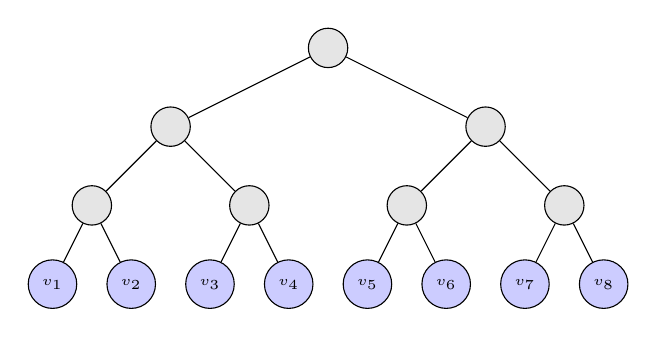
\begin{tikzpicture}[
    level distance=1cm,
    level 1/.style={sibling distance=4cm},
    level 2/.style={sibling distance=2cm},
    level 3/.style={sibling distance=1cm},
    inner/.style={circle, draw, fill=gray!20, minimum size=0.5cm, font=\tiny},
    leaf/.style={circle, draw, fill=blue!20, minimum size=0.5cm, font=\tiny}
]
    \node[inner] (root) {}
        child {
            node[inner] {}
            child {
                node[inner] {}
                child { node[leaf] {$v_1$} }
                child { node[leaf] {$v_2$} }
            }
            child {
                node[inner] {}
                child { node[leaf] {$v_3$} }
                child { node[leaf] {$v_4$} }
            }
        }
        child {
            node[inner] {}
            child {
                node[inner] {}
                child { node[leaf] {$v_5$} }
                child { node[leaf] {$v_6$} }
            }
            child {
                node[inner] {}
                child { node[leaf] {$v_7$} }
                child { node[leaf] {$v_8$} }
            }
        };
\end{tikzpicture}
\end{center}

Each node $v_j$ has a unique path from the root. For example, $v_5$ is reached by: Root $\to$ Right $\to$ Left $\to$ Left.

\paragraph{Step 2: Turn ``Which Node?'' into a Sequence of ``Left or Right?''}

Instead of asking ``Which of the 8 nodes is the context?'' (8-way choice), we ask:
\begin{enumerate}
    \item ``Is the context in the left or right subtree?'' (2-way choice)
    \item ``Within that subtree, left or right?'' (2-way choice)
    \item ``Within that subtree, left or right?'' (2-way choice)
\end{enumerate}

Three binary questions uniquely identify one of 8 leaves. In general, $\log_2 n$ questions for $n$ nodes.

\paragraph{Step 3: Make Each Binary Decision a Learnable Classifier.}

Here's the clever part. At each internal node of the tree, we place a \textbf{learnable vector} $\vect{u}$. This vector, combined with the target embedding $\vect{y}_i$, determines the probability of going left vs.\ right:

\begin{align*}
P(\text{go left}) &= \sigma(\vect{u}^\top \vect{y}_i) \\
P(\text{go right}) &= 1 - \sigma(\vect{u}^\top \vect{y}_i) = \sigma(-\vect{u}^\top \vect{y}_i)
\end{align*}

where $\sigma(x) = 1/(1+e^{-x})$ is the sigmoid. Note that these two probabilities sum to 1 (valid binary distribution).

\begin{center}
\begin{tikzpicture}[
    inner/.style={circle, draw, fill=gray!20, minimum size=0.8cm},
    child_node/.style={circle, draw, minimum size=0.6cm},
    prob/.style={font=\small, fill=white, inner sep=2pt}
]
    \node[inner] (u) {$\vect{u}$};
    \node[child_node, below left=1.2cm and 1.5cm of u] (L) {L};
    \node[child_node, below right=1.2cm and 1.5cm of u] (R) {R};
    
    \draw[-{Stealth}, thick, blue] (u) -- (L) node[midway, prob, left] {$\sigma(\vect{u}^\top \vect{y}_i)$};
    \draw[-{Stealth}, thick, red] (u) -- (R) node[midway, prob, right] {$\sigma(-\vect{u}^\top \vect{y}_i)$};
    
    \node[below=0.3cm of L, font=\small, blue] {left subtree};
    \node[below=0.3cm of R, font=\small, red] {right subtree};
\end{tikzpicture}
\end{center}

\begin{intuition}
\textbf{What's fixed vs.\ what depends on $v_i$?}

\begin{itemize}
    \item \textbf{Fixed (independent of $v_i$)}: The tree structure itself. Node $v_5$ is always reached by the path Root $\to$ Right $\to$ Left $\to$ Left, regardless of who the target is.
    
    \item \textbf{Depends on $v_i$}: The \emph{probability} of taking each branch. The target embedding $\vect{y}_i$ interacts with the internal vectors $\vect{u}$ to determine how likely each path is.
\end{itemize}

\textbf{Analogy}: Think of the tree as a fixed maze, and $\vect{y}_i$ as your ``personality.'' The maze layout doesn't change, but your personality determines how likely you are to turn left or right at each junction. Different targets $v_i$ have different ``personalities'' $\vect{y}_i$, so they have different probabilities of reaching each leaf---even though the maze is the same!
\end{intuition}

\paragraph{Step 4: Multiply the Probabilities Along the Path.}

The probability of reaching a specific leaf is the \textbf{product} of all the binary decisions along the path. This is just the chain rule of probability!

\begin{example}
Let's compute $P(v_5 \mid v_i)$ step by step. The path to $v_5$ is: Root $\to$ Right $\to$ Left $\to$ Left.

\begin{center}
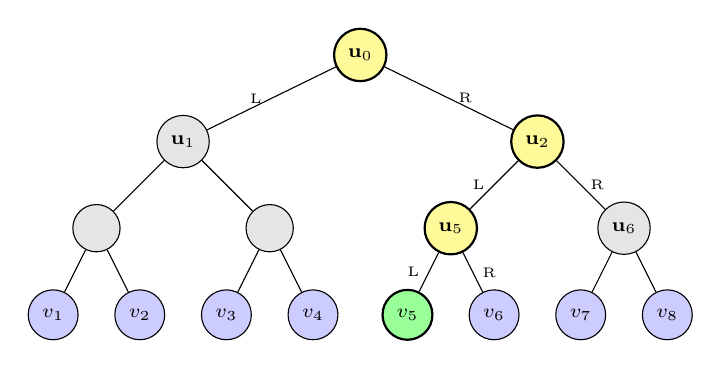
\begin{tikzpicture}[
    level distance=1.1cm,
    level 1/.style={sibling distance=4.5cm},
    level 2/.style={sibling distance=2.2cm},
    level 3/.style={sibling distance=1.1cm},
    inner/.style={circle, draw, fill=gray!20, minimum size=0.6cm, font=\scriptsize},
    inner_highlight/.style={circle, draw, fill=yellow!40, minimum size=0.6cm, font=\scriptsize, thick},
    leaf/.style={circle, draw, fill=blue!20, minimum size=0.6cm, font=\scriptsize},
    leaf_highlight/.style={circle, draw, fill=green!40, minimum size=0.6cm, font=\scriptsize, thick}
]
    \node[inner_highlight] {$\vect{u}_0$}
        child {
            node[inner] {$\vect{u}_1$}
            child {
                node[inner] {}
                child { node[leaf] {$v_1$} edge from parent }
                child { node[leaf] {$v_2$} edge from parent }
                edge from parent
            }
            child {
                node[inner] {}
                child { node[leaf] {$v_3$} edge from parent }
                child { node[leaf] {$v_4$} edge from parent }
                edge from parent
            }
            edge from parent node[left, font=\tiny] {L}
        }
        child {
            node[inner_highlight] {$\vect{u}_2$}
            child {
                node[inner_highlight] {$\vect{u}_5$}
                child { node[leaf_highlight] {$v_5$} edge from parent node[left, font=\tiny] {L} }
                child { node[leaf] {$v_6$} edge from parent node[right, font=\tiny] {R} }
                edge from parent node[left, font=\tiny] {L}
            }
            child {
                node[inner] {$\vect{u}_6$}
                child { node[leaf] {$v_7$} edge from parent }
                child { node[leaf] {$v_8$} edge from parent }
                edge from parent node[right, font=\tiny] {R}
            }
            edge from parent node[right, font=\tiny] {R}
        };
\end{tikzpicture}
\end{center}

The computation:
\begin{align*}
P(v_5 \mid v_i) &= P(\text{Right at } \vect{u}_0) \times P(\text{Left at } \vect{u}_2) \times P(\text{Left at } \vect{u}_5) \\[0.5em]
&= \underbrace{\sigma(-\vect{u}_0^\top \vect{y}_i)}_{\text{go right}} \times \underbrace{\sigma(+\vect{u}_2^\top \vect{y}_i)}_{\text{go left}} \times \underbrace{\sigma(+\vect{u}_5^\top \vect{y}_i)}_{\text{go left}}
\end{align*}

\textbf{Total cost}: 3 dot products and 3 sigmoids (instead of 8 exponentials + sum for regular softmax).
\end{example}

\begin{remark}[What Depends on What?]
A common point of confusion: the \textbf{tree structure is fixed}---node $v_5$ is always reached by the path Root $\to$ Right $\to$ Left $\to$ Left, regardless of the target node.

But the \textbf{probabilities at each branch depend on $v_i$}! For two different target nodes:
\begin{align*}
P(v_5 \mid v_i) &= \sigma(-\vect{u}_0^\top \textcolor{blue}{\vect{y}_i}) \cdot \sigma(\vect{u}_2^\top \textcolor{blue}{\vect{y}_i}) \cdot \sigma(\vect{u}_5^\top \textcolor{blue}{\vect{y}_i}) \\
P(v_5 \mid v_k) &= \sigma(-\vect{u}_0^\top \textcolor{red}{\vect{y}_k}) \cdot \sigma(\vect{u}_2^\top \textcolor{red}{\vect{y}_k}) \cdot \sigma(\vect{u}_5^\top \textcolor{red}{\vect{y}_k})
\end{align*}
These give different probabilities because the embeddings $\vect{y}_i$ and $\vect{y}_k$ are different.

\textbf{Intuition}: The tree defines the ``questions'' (left or right at each internal node), but the target embedding $\vect{y}_i$ determines the ``answers'' (the probability of each direction).
\end{remark}

\paragraph{Why Do the Probabilities Sum to 1?}

This is crucial for hierarchical softmax to define a valid probability distribution. Here's why it works:

At each internal node, probabilities of left and right sum to 1:
\[
P(\text{left}) + P(\text{right}) = \sigma(\vect{u}^\top \vect{y}_i) + \sigma(-\vect{u}^\top \vect{y}_i) = 1
\]

Now consider all 8 leaves. We can group them by the first decision:
\begin{align*}
\sum_{j=1}^{8} P(v_j \mid v_i) &= \underbrace{P(\text{left at root}) \times (\text{sum over } v_1, v_2, v_3, v_4)}_{\text{left subtree}} + \underbrace{P(\text{right at root}) \times (\text{sum over } v_5, v_6, v_7, v_8)}_{\text{right subtree}}
\end{align*}

By induction, each subtree's probabilities sum to 1 (conditioned on reaching that subtree). So the total is:
\[
P(\text{left}) \times 1 + P(\text{right}) \times 1 = 1 \quad \checkmark
\]

\paragraph{The Formal Definition (Now It Should Make Sense!)}

\begin{definition}[Hierarchical Softmax]
Let each node $v_j$ be a leaf in a binary tree, with path $(\pi_0, \pi_1, \ldots, \pi_{L_j})$ from root to $v_j$. Each internal node $\pi_\ell$ has a learnable vector $\vect{u}_{\pi_\ell}$. Then:
\[
P(v_j \mid v_i) = \prod_{\ell=0}^{L_j - 1} \sigma\bigl(s_\ell \cdot \vect{u}_{\pi_\ell}^\top \vect{y}_i\bigr)
\]
where $s_\ell = +1$ if the path goes left at $\pi_\ell$, and $s_\ell = -1$ if it goes right.
\end{definition}

\begin{intuition}
\textbf{Summary}: Hierarchical softmax replaces one $n$-way classification with $\log n$ binary classifications. Each binary classifier asks ``left or right?'' based on the target embedding $\vect{y}_i$ and a learned vector $\vect{u}$ at that tree node. The final probability is the product of all binary decisions along the path to the context node.
\end{intuition}

\begin{keyinsight}
\textbf{Comparing the two approaches}:

\begin{center}
\begin{tabular}{lcc}
\toprule
 & \textbf{Negative Sampling} & \textbf{Hierarchical Softmax} \\
\midrule
Cost per update & $O(K)$ & $O(\log n)$ \\
What's learned & Node embeddings $\vect{y}_i$ & Node embeddings $\vect{y}_i$ + tree vectors $\vect{u}_k$ \\
Probability & Approximation & Exact (but different model) \\
Hyperparameters & $K$ (num.\ negatives) & Tree structure \\
Better for & Frequent nodes & Rare nodes \\
\bottomrule
\end{tabular}
\end{center}

\textbf{In practice}: Negative sampling is more commonly used because:
\begin{itemize}
    \item Simpler to implement
    \item Often gives comparable or better results
    \item The original DeepWalk paper used hierarchical softmax, but Node2Vec and most subsequent work use negative sampling
\end{itemize}
\end{keyinsight}

\begin{remark}[How is the Tree Constructed?]
The tree structure matters! Common choices:
\begin{itemize}
    \item \textbf{Huffman tree}: Frequent nodes get shorter paths (closer to root). This is what word2vec uses---frequent words need fewer computations.
    \item \textbf{Random balanced tree}: Simple but not optimal.
    \item \textbf{Semantic tree}: Cluster similar nodes into subtrees (rarely used in practice).
\end{itemize}
For graphs, a Huffman tree based on node degree (high-degree nodes closer to root) is a reasonable choice.
\end{remark}

\subsection{DeepWalk}

\begin{definition}[DeepWalk]
DeepWalk = Random Walks + Skip-Gram
\begin{enumerate}
    \item Generate $\gamma$ random walks of length $\ell$ starting from each node
    \item Train a skip-gram model on the resulting ``corpus'' of walks
\end{enumerate}
\end{definition}

\begin{algorithm}
\caption{DeepWalk}
\begin{algorithmic}[1]
\Require Graph $G$, walks per node $\gamma$, walk length $\ell$, embedding dim $d$, window $c$
\State Initialize embeddings randomly
\For{$i = 1$ to $\gamma$}
    \For{each node $v \in V$}
        \State $W \gets \text{RandomWalk}(G, v, \ell)$ \Comment{e.g., $[v, u_1, u_2, \ldots]$}
        \State Update embeddings using Skip-Gram on $W$
    \EndFor
\EndFor
\State \Return embeddings $\embed$
\end{algorithmic}
\end{algorithm}

\begin{example}
Let's trace DeepWalk on our graph.

\textbf{Step 1: Generate random walks} (say, $\gamma=2$ walks per node, $\ell=4$)

Starting from node 1:
\begin{itemize}
    \item Walk 1: $1 \to 2 \to 3 \to 1 \to 2$ (randomly chose neighbors)
    \item Walk 2: $1 \to 3 \to 2 \to 4 \to 5$
\end{itemize}

Starting from node 4:
\begin{itemize}
    \item Walk 1: $4 \to 2 \to 1 \to 3 \to 2$
    \item Walk 2: $4 \to 6 \to 5 \to 4 \to 2$
\end{itemize}

\textbf{Step 2: Extract training pairs} (window $c=1$)

From walk $[1, 2, 3, 1, 2]$:
\begin{center}
\begin{tabular}{cc}
\toprule
Target & Context \\
\midrule
1 & 2 \\
2 & 1, 3 \\
3 & 2, 1 \\
1 & 3, 2 \\
\bottomrule
\end{tabular}
\end{center}

\textbf{Step 3: Train skip-gram}

For pair (target=2, context=3): increase $\vect{y}_2^\top \vect{y}_3$

For negative sample (target=2, negative=6): decrease $\vect{y}_2^\top \vect{y}_6$

After many iterations, nodes that frequently co-occur in walks will have similar embeddings!
\end{example}

\subsubsection*{The Deep Connection: Skip-Gram is Matrix Factorization!}

At first glance, DeepWalk (random walks + skip-gram) seems completely different from the matrix factorization methods we saw earlier (GF, HOPE, GraRep). One uses neural network training with stochastic gradient descent; the other uses linear algebra (SVD).

\begin{whybox}
But here's a remarkable fact: \textbf{they're secretly doing the same thing!} 

A beautiful theoretical result shows that skip-gram with negative sampling implicitly factorizes a specific matrix. This explains why DeepWalk works so well---it's not just a heuristic, it has solid mathematical foundations.
\end{whybox}

\begin{theorem}[What Does DeepWalk Actually Learn? {\cite{shallow-embeddings:qiu2018}}]
When trained to convergence, DeepWalk's embeddings satisfy $\embed \embed^\top \approx \mathbf{M}$, where:
\[
\mathbf{M} = \log\left(\frac{\text{vol}(G)}{c} \sum_{r=1}^{c} \transition^r \degree^{-1}\right) - \log K
\]
Here:
\begin{itemize}
    \item $\transition = \degree^{-1}\adj$ is the random walk transition matrix
    \item $c$ is the context window size
    \item $K$ is the number of negative samples
    \item $\text{vol}(G) = \sum_i d_i$ is the total degree (twice the number of edges)
\end{itemize}
\end{theorem}

\begin{intuition}
Let's unpack what this matrix $\mathbf{M}$ captures:

\begin{itemize}
    \item $\transition^r$ is the $r$-step random walk probability matrix (we saw this in GraRep!)
    \item $\sum_{r=1}^{c} \transition^r$ averages over all path lengths from 1 to $c$
    \item The $\log$ transformation converts probabilities to PMI-like quantities (just like GraRep!)
    \item The $\degree^{-1}$ term normalizes by node popularity
\end{itemize}

\textbf{In other words}: DeepWalk is approximately factorizing a matrix that looks a lot like what GraRep explicitly constructs! The random walks and skip-gram training are just a clever, scalable way to achieve the same goal.
\end{intuition}

\begin{keyinsight}
This theorem has profound implications:

\begin{enumerate}
    \item \textbf{Unification}: Skip-gram methods and matrix factorization methods are two sides of the same coin
    \item \textbf{The Laplacian appears again}: Since $\transition = \identity - \lamark_{\text{rw}}$, DeepWalk implicitly encodes spectral information about the graph
    \item \textbf{Design insights}: Want to capture longer-range structure? Increase window size $c$. Want sharper embeddings? Increase negative samples $K$.
\end{enumerate}
\end{keyinsight}

\subsection{Node2Vec: Controlling the Random Walk}

\begin{whybox}
DeepWalk uses uniform random walks. But sometimes we want more control:
\begin{itemize}
    \item \textbf{Homophily}: Nodes nearby in the graph should be similar (DFS-like exploration)
    \item \textbf{Structural equivalence}: Nodes with similar roles should be similar (BFS-like, stay local)
\end{itemize}
Node2Vec lets us interpolate between these!
\end{whybox}

\begin{definition}[Biased Random Walk in Node2Vec]
Suppose the walk just traversed edge $(t, v)$, so we're now at node $v$ having come from node $t$. To choose the next node $x$, we can only go to neighbors of $v$. The transition probability depends on the relationship between $x$ and the \emph{previous} node $t$:
\[
P(v \to x \mid t \to v) \propto \alpha_{pq}(t, x) = \begin{cases}
    1/p & \text{if } x = t \text{ (return to previous node)} \\
    1 & \text{if } x \neq t \text{ and } x \in \mathcal{N}(t) \text{ (}x\text{ is also neighbor of }t\text{)} \\
    1/q & \text{if } x \neq t \text{ and } x \notin \mathcal{N}(t) \text{ (}x\text{ moves away from }t\text{)}
\end{cases}
\]
where $\mathcal{N}(t)$ denotes the neighbors of $t$. The actual probability is obtained by normalizing over all neighbors of $v$:
\[
P(v \to x \mid t \to v) = \frac{\alpha_{pq}(t,x)}{\sum_{x' \in \mathcal{N}(v)} \alpha_{pq}(t, x')}
\]
\end{definition}

\begin{figure}[htbp]
\centering
\begin{tikzpicture}[
    node distance=1.5cm and 2cm,
    % Styles
    main/.style={circle, draw, thick, minimum size=0.9cm, font=\small\bfseries},
    prob/.style={font=\footnotesize, inner sep=2pt, fill=white, rounded corners=2pt},
    arrow/.style={-{Stealth[scale=1.2]}, very thick}
]
    % Nodes
    \node[main, fill=gray!20, label=below:previous] (t) {$t$};
    \node[main, fill=yellow!30, right=of t, label=below:current] (v) {$v$};
    
    % Neighbors
    \node[main, fill=blue!10, above right=1.1cm and 2cm of v] (x1) {$x_1$};
    \node[main, fill=green!10, right=2.5cm of v] (x2) {$x_2$};
    \node[main, fill=red!10, below right=1.1cm and 2cm of v] (x3) {$x_3$};
    
    % Structural Undirected Edges
    \draw[thick, gray] (t) -- (v);
    \draw[thick, gray] (v) -- (x1);
    \draw[thick, gray] (v) -- (x2);
    \draw[thick, gray] (v) -- (x3);
    \draw[thick, gray] (t) to[bend left=40] (x1); % Neighbor connection
    
    % Transition Probabilities (Directed)
    \begin{scope}[every node/.style={prob}]
        % Return to t
        \draw[arrow, blue] (v) to[bend left] node {$1/p$} (t);
        
        % Move to neighbor of t
        \draw[arrow, green!60!black] (v) to[bend left=15] node {$1$} (x1);
        
        % Move away from t
        \draw[arrow, red] (v) to[bend right=-15] node[above] {$1/q$} (x2);
        \draw[arrow, red] (v) to[bend right=-15] node[above] {$1/q$} (x3);
    \end{scope}
    
    % Legend (Boxed for clarity)
    \node[draw, rounded corners, right=1cm of x2, font=\small, inner sep=6pt] (legend) {
        \begin{tabular}{ll}
            \textcolor{blue}{$\bullet$ $x = t$} & \textcolor{blue}{return ($1/p$)} \\
            \textcolor{green!60!black}{$\bullet$ $x \in \mathcal{N}(t)$} & \textcolor{green!60!black}{neighbor ($1$)} \\
            \textcolor{red}{$\bullet$ $x \notin \mathcal{N}(t)$} & \textcolor{red}{away ($1/q$)}
        \end{tabular}
    };
\end{tikzpicture}
\caption{Node2Vec biased random walk. From $v$ (having come from $t$), transition probabilities depend on distance to previous node $t$.}
\label{shallow-embeddings:fig:node2vec_walk}
\end{figure}

\begin{example}
On our graph, consider a walk that just moved from node 2 to node 4. So $t = 2$ (previous) and $v = 4$ (current).

From node 4, the neighbors are: $\mathcal{N}(4) = \{2, 5, 6\}$

For each possible next node $x \in \mathcal{N}(4)$, we compute the unnormalized weight $\alpha_{pq}(t, x)$:
\begin{itemize}
    \item $x = 2$: This is returning to $t$, so $\alpha_{pq}(2, 2) = 1/p$
    \item $x = 5$: Is $5 \in \mathcal{N}(2)$? Node 2's neighbors are $\{1, 3, 4\}$, so no. Thus $\alpha_{pq}(2, 5) = 1/q$
    \item $x = 6$: Is $6 \in \mathcal{N}(2)$? No. Thus $\alpha_{pq}(2, 6) = 1/q$
\end{itemize}

\textbf{Case 1:} $p=1, q=2$ (encourage returning, discourage exploring)
\begin{align*}
\alpha_{pq}(2,2) &= 1/1 = 1, \quad \alpha_{pq}(2,5) = \alpha_{pq}(2,6) = 1/2 = 0.5 \\
Z &= 1 + 0.5 + 0.5 = 2 \\
P(4 \to 2) &= 1/2 = 0.5, \quad P(4 \to 5) = P(4 \to 6) = 0.5/2 = 0.25
\end{align*}

\textbf{Case 2:} $p=2, q=0.5$ (discourage returning, encourage exploring)
\begin{align*}
\alpha_{pq}(2,2) &= 1/2 = 0.5, \quad \alpha_{pq}(2,5) = \alpha_{pq}(2,6) = 1/0.5 = 2 \\
Z &= 0.5 + 2 + 2 = 4.5 \\
P(4 \to 2) &= 0.5/4.5 \approx 0.11, \quad P(4 \to 5) = P(4 \to 6) = 2/4.5 \approx 0.44
\end{align*}

The second setting pushes the walk deeper into community B (away from where it came from)!
\end{example}

\begin{keyinsight}
\textbf{Choosing $p$ and $q$}:
\begin{itemize}
    \item \textbf{Low $p$}: Encourage returning → very local exploration (BFS-like)
    \item \textbf{High $p$}: Discourage returning → keep moving forward
    \item \textbf{Low $q$}: Encourage moving to new areas → DFS-like, captures homophily
    \item \textbf{High $q$}: Stay close to starting region → BFS-like, captures structural equivalence
\end{itemize}

\textbf{Rule of thumb}: 
\begin{itemize}
    \item For community detection: use low $q$ (explore communities deeply)
    \item For role detection (hubs, bridges): use high $q$ (stay local, see structure)
\end{itemize}
\end{keyinsight}

\begin{figure}[htbp]
\centering
\begin{tikzpicture}
    % BFS-like
    \begin{scope}[xshift=0cm]
        \node[font=\bfseries] at (1.5, 2.5) {High $q$ (BFS-like)};
        \node[circle, draw, fill=yellow!50, minimum size=0.5cm] (c) at (1.5, 1) {};
        \foreach \angle/\col in {0/blue!30, 60/blue!30, 120/blue!30, 180/blue!30, 240/blue!30, 300/blue!30} {
            \node[circle, draw, fill=\col, minimum size=0.4cm] (n\angle) at ($(c) + (\angle:0.8cm)$) {};
            \draw (c) -- (n\angle);
        }
        \node[below of=c, yshift=-0.3cm, font=\small] {Explores neighborhood};
    \end{scope}
    
    % DFS-like
    \begin{scope}[xshift=5cm]
        \node[font=\bfseries] at (1.5, 2.5) {Low $q$ (DFS-like)};
        \node[circle, draw, fill=yellow!50, minimum size=0.5cm] (c2) at (0, 1) {};
        \node[circle, draw, fill=green!30, minimum size=0.4cm] (n1) at (1, 1) {};
        \node[circle, draw, fill=green!30, minimum size=0.4cm] (n2) at (2, 1) {};
        \node[circle, draw, fill=green!30, minimum size=0.4cm] (n3) at (3, 1) {};
        \draw (c2) -- (n1) -- (n2) -- (n3);
        \node[below of=n1, yshift=0.1cm, xshift=0.5cm, font=\small] {Goes deeper};
    \end{scope}
\end{tikzpicture}
\caption{Different walk strategies: BFS-like (high $q$) stays local; DFS-like (low $q$) explores further.}
\label{shallow-embeddings:fig:bfs_dfs}
\end{figure}


% ============================================================================
% SECTION 5: MULTI-RELATIONAL GRAPHS AND KNOWLEDGE GRAPH EMBEDDINGS
% ============================================================================
\section{Multi-Relational Graphs and Knowledge Graph Embeddings}

So far, we have considered \textbf{simple graphs} where edges are homogeneous---all edges represent the same type of relationship. However, many real-world graphs have \textbf{multiple types of relationships} between nodes. This section develops the theory of embedding such \emph{multi-relational graphs}, with a particular focus on \emph{knowledge graphs}.

\subsection{What Are Multi-Relational Graphs?}

\begin{whybox}
Consider these scenarios where a single edge type is insufficient:
\begin{itemize}
    \item \textbf{Social networks}: Alice can be Bob's ``friend,'' ``colleague,'' or ``spouse''---these are fundamentally different relationships
    \item \textbf{Biomedical networks}: A drug can ``treat'' a disease, ``cause'' a side effect, or ``interact with'' another drug
    \item \textbf{Knowledge bases}: We might know that (Einstein, \textsc{BornIn}, Germany), (Einstein, \textsc{WonAward}, NobelPrize), (Einstein, \textsc{WorkedAt}, Princeton)
\end{itemize}
A simple adjacency matrix $\adj$ cannot capture these distinctions!
\end{whybox}

\begin{definition}[Multi-Relational Graph]
A \textbf{multi-relational graph} is a tuple $\mathcal{G} = (V, E, \mathcal{R})$ where:
\begin{itemize}
    \item $V = \{v_1, \ldots, v_n\}$ is the set of \textbf{nodes} (also called \emph{entities})
    \item $\mathcal{R} = \{\tau_1, \ldots, \tau_R\}$ is the set of \textbf{relation types}
    \item $E \subseteq V \times \mathcal{R} \times V$ is the set of \textbf{edges} (also called \emph{triples} or \emph{facts})
\end{itemize}
Each edge is a triple $e = (u, \tau, v)$ indicating that relation $\tau$ holds from node $u$ to node $v$.
\end{definition}

\begin{intuition}
We can think of a multi-relational graph as having $R$ different ``layers,'' one for each relation type. Alternatively, we can represent it as a 3D \textbf{adjacency tensor} $\mathcal{A} \in \{0,1\}^{n \times R \times n}$ where:
\[
\mathcal{A}[u, \tau, v] = \begin{cases} 1 & \text{if } (u, \tau, v) \in E \\ 0 & \text{otherwise} \end{cases}
\]
\end{intuition}

\begin{figure}[htbp]
\centering
\begin{tikzpicture}[
    node distance=2cm,
    entity/.style={circle, draw, thick, minimum size=1cm, font=\small\bfseries, fill=white},
    rel/.style={font=\small\itshape, fill=white, inner sep=2pt}
]
    % Entities
    \node[entity, fill=node1color!30] (einstein) {Einstein};
    \node[entity, fill=node3color!30, right=3.5cm of einstein] (germany) {Germany};
    \node[entity, fill=node2color!30, below=2cm of einstein] (nobel) {Nobel};
    \node[entity, fill=node4color!30, below=2cm of germany] (physics) {Physics};
    
    % Relations with different colors for different types
    \draw[-{Stealth}, thick, blue!70] (einstein) -- node[rel, above] {\textsc{BornIn}} (germany);
    \draw[-{Stealth}, thick, red!70] (einstein) -- node[rel, left] {\textsc{Won}} (nobel);
    \draw[-{Stealth}, thick, green!60!black] (einstein) -- node[rel, above, sloped] {\textsc{FieldOf}} (physics);
    \draw[-{Stealth}, thick, orange!80] (nobel) -- node[rel, below] {\textsc{Category}} (physics);
    
    % Legend
    \node[draw, rounded corners, right=0.5cm of germany, yshift=-2cm, font=\small] {
        \begin{tabular}{l}
            \textcolor{blue!70}{\textsc{BornIn}} \\
            \textcolor{red!70}{\textsc{Won}} \\
            \textcolor{green!60!black}{\textsc{FieldOf}} \\
            \textcolor{orange!80}{\textsc{Category}}
        \end{tabular}
    };
\end{tikzpicture}
\caption{A small knowledge graph with multiple relation types. Each arrow represents a different kind of relationship.}
\label{shallow-embeddings:fig:knowledge_graph}
\end{figure}

\begin{definition}[Knowledge Graph]
A \textbf{knowledge graph} is a multi-relational graph where:
\begin{itemize}
    \item Nodes represent real-world \textbf{entities} (people, places, concepts, etc.)
    \item Edges represent \textbf{facts} about relationships between entities
    \item Each triple $(h, \tau, t)$ can be read as ``\emph{head} has relation $\tau$ to \emph{tail}''
\end{itemize}
Common notation: $(h, r, t)$ for (head, relation, tail), emphasizing the directed nature.
\end{definition}

\begin{example}
Some well-known knowledge graphs include:
\begin{itemize}
    \item \textbf{Freebase}: 1.9 billion triples about general knowledge
    \item \textbf{WordNet}: Semantic relationships between English words
    \item \textbf{YAGO}: Facts extracted from Wikipedia and WordNet
    \item \textbf{Wikidata}: Collaborative knowledge base with 100M+ items
\end{itemize}
A typical knowledge graph might have $n \sim 10^6$ entities, $R \sim 10^3$ relations, and $|E| \sim 10^8$ triples.
\end{example}

\subsection{The Knowledge Graph Completion Problem}

\begin{whybox}
Knowledge graphs are inherently \textbf{incomplete}---they contain only a fraction of all true facts. For example, Freebase is missing 71\% of person birthplaces and 75\% of nationalities! The task of \textbf{knowledge graph completion} (or \emph{link prediction}) is to predict missing edges.
\end{whybox}

\begin{definition}[Knowledge Graph Completion]
Given a knowledge graph $\mathcal{G} = (V, E, \mathcal{R})$, the goal is to predict whether a candidate triple $(h, \tau, t) \notin E$ is likely to be a true fact.

Formally, we want to learn a \textbf{scoring function} $f: V \times \mathcal{R} \times V \to \R$ such that:
\[
f(h, \tau, t) > f(h', \tau', t') \quad \text{when } (h, \tau, t) \text{ is more likely to be true}
\]
\end{definition}

\begin{intuition}
This is exactly the link prediction problem, but now we must also predict the \emph{type} of link! The challenge is that different relation types have very different semantics:
\begin{itemize}
    \item \textsc{BornIn} is many-to-one (many people born in one city)
    \item \textsc{Spouse} is one-to-one (ideally!)
    \item \textsc{HasCitizen} is one-to-many (one country, many citizens)
    \item \textsc{Colleague} is symmetric; \textsc{Supervises} is antisymmetric
\end{itemize}
Our embedding methods must capture these diverse patterns.
\end{intuition}

\subsection{The Encoder-Decoder Framework for Multi-Relational Data}

We extend the encoder-decoder framework from simple graphs to multi-relational graphs.

\begin{definition}[Multi-Relational Encoder]
The encoder maps each entity $v \in V$ to an embedding vector:
\[
\text{enc}: V \to \R^d, \quad v \mapsto \vect{z}_v
\]
For shallow embeddings, this is simply a lookup: $\text{enc}(v) = \vect{Z}[v]$ where $\vect{Z} \in \R^{n \times d}$ is the embedding matrix.

Additionally, we must encode the \textbf{relation types}. Different methods do this differently---some use relation vectors $\vect{r}_\tau \in \R^d$, others use relation matrices $\vect{R}_\tau \in \R^{d \times d}$.
\end{definition}

\begin{definition}[Multi-Relational Decoder]
The decoder takes entity embeddings and a relation type to produce a score:
\[
\text{dec}: \R^d \times \mathcal{R} \times \R^d \to \R, \quad (\vect{z}_h, \tau, \vect{z}_t) \mapsto f(h, \tau, t)
\]
The score $f(h, \tau, t)$ should be high for true triples and low for false ones.
\end{definition}

\begin{keyinsight}
The key distinction from simple graph embedding is that the decoder is now \textbf{relation-specific}. We can't just use $\vect{z}_h^\top \vect{z}_t$ because:
\begin{enumerate}
    \item It ignores the relation type entirely
    \item It's symmetric, but many relations are not
    \item Different relations require different notions of ``similarity''
\end{enumerate}
The art of knowledge graph embedding lies in designing decoders that capture the semantics of diverse relation types.
\end{keyinsight}

\subsection{Loss Functions for Multi-Relational Embedding}

Before diving into specific decoders, let's establish the loss functions used to train these models.

\subsubsection*{The Naive Reconstruction Loss (and Why It's Impractical)}

One might try to directly minimize reconstruction error over all possible triples:
\[
\mathcal{L}_{\text{naive}} = \sum_{h \in V} \sum_{\tau \in \mathcal{R}} \sum_{t \in V} \ell\bigl(\text{dec}(\vect{z}_h, \tau, \vect{z}_t), \mathcal{A}[h, \tau, t]\bigr)
\]

\begin{whybox}
This is computationally infeasible! The sum has $O(n^2 R)$ terms. For a knowledge graph with $n = 10^6$ entities and $R = 10^3$ relations, that's $10^{15}$ terms per gradient step. We need smarter approaches.
\end{whybox}

\subsubsection*{Cross-Entropy Loss with Negative Sampling}

The most common approach uses \textbf{negative sampling}, similar to what we saw for DeepWalk:

\begin{definition}[Cross-Entropy Loss with Negative Sampling]
For each true triple $(h, \tau, t) \in E$:
\begin{enumerate}
    \item Generate $K$ \textbf{negative samples} by corrupting either the head or tail:
    \[
    (h', \tau, t) \text{ where } h' \sim P_n(V), \quad \text{or} \quad (h, \tau, t') \text{ where } t' \sim P_n(V)
    \]
    \item Maximize the score gap between positive and negative triples
\end{enumerate}

The loss function is:
\begin{align}
\mathcal{L}_{\text{CE}} = \sum_{(h,\tau,t) \in E} \Bigl[ 
&-\log \sigma\bigl(\text{dec}(\vect{z}_h, \tau, \vect{z}_t)\bigr) \nonumber \\
&- \frac{1}{K}\sum_{k=1}^{K} \log \sigma\bigl(-\text{dec}(\vect{z}_{h_k'}, \tau, \vect{z}_t)\bigr) \nonumber \\
&- \frac{1}{K}\sum_{k=1}^{K} \log \sigma\bigl(-\text{dec}(\vect{z}_h, \tau, \vect{z}_{t_k'})\bigr)
\Bigr]
\end{align}
where $\sigma(x) = 1/(1+e^{-x})$ is the sigmoid function.
\end{definition}

\begin{intuition}
This loss has three parts:
\begin{enumerate}
    \item \textbf{Positive term}: Push $\text{dec}(\vect{z}_h, \tau, \vect{z}_t)$ to be large (so $\sigma(\cdot) \approx 1$)
    \item \textbf{Head corruption}: Push $\text{dec}(\vect{z}_{h'}, \tau, \vect{z}_t)$ to be small for random $h'$
    \item \textbf{Tail corruption}: Push $\text{dec}(\vect{z}_h, \tau, \vect{z}_{t'})$ to be small for random $t'$
\end{enumerate}
Complexity: $O(|E| \cdot K)$ per epoch, which is tractable!
\end{intuition}

\subsubsection*{Max-Margin Loss (Hinge Loss)}

An alternative is the \textbf{margin-based ranking loss}:

\begin{definition}[Max-Margin Loss]
\begin{equation}
\mathcal{L}_{\text{margin}} = \sum_{(h,\tau,t) \in E} \sum_{(h',\tau,t') \in \mathcal{N}_{h,\tau,t}} \max\Bigl(0, \gamma + \text{dec}(\vect{z}_{h'}, \tau, \vect{z}_{t'}) - \text{dec}(\vect{z}_h, \tau, \vect{z}_t)\Bigr)
\end{equation}
where:
\begin{itemize}
    \item $\mathcal{N}_{h,\tau,t}$ is the set of negative samples for triple $(h, \tau, t)$
    \item $\gamma > 0$ is the \textbf{margin} hyperparameter
\end{itemize}
\end{definition}

\begin{intuition}
The loss is zero when the true triple's score exceeds all negative samples' scores by at least $\gamma$. Otherwise, we incur a penalty proportional to the violation.

\textbf{Comparison with cross-entropy}:
\begin{itemize}
    \item Cross-entropy: Works with probabilities (via sigmoid), smoother gradients
    \item Margin loss: Works with raw scores, focuses on ranking rather than calibration
\end{itemize}
Both are widely used; the choice often depends on the decoder.
\end{intuition}

\begin{remark}[Negative Sampling Strategies]
The quality of negative samples significantly impacts learning:
\begin{itemize}
    \item \textbf{Uniform}: Sample $h'$ or $t'$ uniformly from $V$. Simple but may produce ``easy'' negatives.
    \item \textbf{Frequency-based}: Sample proportional to entity frequency, like $P_n(v) \propto (\text{freq}(v))^{3/4}$
    \item \textbf{Type-constrained}: Only sample entities of the correct type (e.g., for \textsc{BornIn}, only sample locations as tails)
    \item \textbf{Adversarial}: Use a separate model to generate hard negatives
\end{itemize}
Filtering known positives from the negative sample set (``filtered'' setting) is important for evaluation.
\end{remark}


\subsection{Multi-Relational Decoders: A Comprehensive Treatment}

We now present the main decoder architectures, organized by their underlying mathematical principles.

\subsubsection{Bilinear Models: RESCAL and Its Descendants}

The earliest and most general approach uses \textbf{bilinear forms} to model relation-specific interactions.

\begin{definition}[RESCAL Decoder]
Each relation $\tau$ is associated with a \textbf{relation matrix} $\vect{R}_\tau \in \R^{d \times d}$:
\begin{equation}
f_{\text{RESCAL}}(h, \tau, t) = \vect{z}_h^\top \vect{R}_\tau \vect{z}_t = \sum_{i=1}^{d} \sum_{j=1}^{d} z_{h,i} \cdot R_{\tau,ij} \cdot z_{t,j}
\end{equation}
\end{definition}

\begin{mathbox}
\textbf{Understanding the Bilinear Form}

Let's unpack what $\vect{z}_h^\top \vect{R}_\tau \vect{z}_t$ computes. If we write out the matrix multiplication:
\[
\vect{z}_h^\top \vect{R}_\tau \vect{z}_t = \sum_{i=1}^{d} \sum_{j=1}^{d} z_{h,i} \cdot R_{\tau,ij} \cdot z_{t,j}
\]

Each entry $R_{\tau,ij}$ controls how the $i$-th dimension of the head interacts with the $j$-th dimension of the tail \emph{for this specific relation}.

\textbf{Special cases}:
\begin{itemize}
    \item If $\vect{R}_\tau = \vect{I}$ (identity), we recover the simple inner product $\vect{z}_h^\top \vect{z}_t$
    \item If $\vect{R}_\tau = \text{diag}(\vect{r}_\tau)$ is diagonal, we get DistMult (see below)
    \item If $\vect{R}_\tau$ is symmetric, the decoder is symmetric: $f(h, \tau, t) = f(t, \tau, h)$
\end{itemize}
\end{mathbox}

\begin{example}
Let $d = 2$ with embeddings:
\[
\vect{z}_{\text{Einstein}} = \begin{pmatrix} 0.8 \\ 0.3 \end{pmatrix}, \quad
\vect{z}_{\text{Germany}} = \begin{pmatrix} 0.2 \\ 0.9 \end{pmatrix}
\]
and relation matrix for \textsc{BornIn}:
\[
\vect{R}_{\textsc{BornIn}} = \begin{pmatrix} 0.5 & 0.1 \\ -0.2 & 0.8 \end{pmatrix}
\]

Then:
\begin{align*}
f(\text{Einstein}, \textsc{BornIn}, \text{Germany}) &= \begin{pmatrix} 0.8 & 0.3 \end{pmatrix} 
\begin{pmatrix} 0.5 & 0.1 \\ -0.2 & 0.8 \end{pmatrix}
\begin{pmatrix} 0.2 \\ 0.9 \end{pmatrix} \\
&= \begin{pmatrix} 0.8 & 0.3 \end{pmatrix} \begin{pmatrix} 0.19 \\ 0.68 \end{pmatrix} \\
&= 0.152 + 0.204 = 0.356
\end{align*}

Note: $f(\text{Germany}, \textsc{BornIn}, \text{Einstein}) = 0.215 \neq 0.356$ because the relation matrix is not symmetric. This allows RESCAL to model asymmetric relations!
\end{example}

\begin{keyinsight}
\textbf{RESCAL's Expressiveness vs.\ Complexity Trade-off}

\textbf{Pros}:
\begin{itemize}
    \item Fully expressive: Can model any relation pattern
    \item Captures complex interactions between embedding dimensions
\end{itemize}

\textbf{Cons}:
\begin{itemize}
    \item $O(d^2)$ parameters \emph{per relation}---for $d = 200$ and $R = 1000$, that's 40 billion relation parameters!
    \item Prone to overfitting on rare relations
    \item Quadratic computation per triple
\end{itemize}

This motivates more efficient variants.
\end{keyinsight}

\begin{definition}[DistMult: Diagonal Bilinear Model]
Restrict $\vect{R}_\tau$ to be diagonal: $\vect{R}_\tau = \text{diag}(\vect{r}_\tau)$ where $\vect{r}_\tau \in \R^d$:
\begin{equation}
f_{\text{DistMult}}(h, \tau, t) = \langle \vect{z}_h, \vect{r}_\tau, \vect{z}_t \rangle = \sum_{i=1}^{d} z_{h,i} \cdot r_{\tau,i} \cdot z_{t,i}
\end{equation}
This is equivalent to element-wise multiplication followed by summation:
\[
f_{\text{DistMult}}(h, \tau, t) = (\vect{z}_h \odot \vect{r}_\tau)^\top \vect{z}_t
\]
where $\odot$ denotes the Hadamard (element-wise) product.
\end{definition}

\begin{mathbox}
\textbf{Why Diagonal Restriction?}

With a diagonal relation matrix:
\[
\vect{z}_h^\top \text{diag}(\vect{r}_\tau) \vect{z}_t = \sum_i z_{h,i} \cdot r_{\tau,i} \cdot z_{t,i}
\]

Each dimension $i$ contributes $z_{h,i} \cdot z_{t,i}$, weighted by $r_{\tau,i}$:
\begin{itemize}
    \item If $r_{\tau,i} > 0$: Dimension $i$ should \emph{match} (positive contribution when $z_{h,i}$ and $z_{t,i}$ have same sign)
    \item If $r_{\tau,i} < 0$: Dimension $i$ should \emph{differ}
    \item If $r_{\tau,i} \approx 0$: Dimension $i$ is irrelevant for this relation
\end{itemize}

The relation vector $\vect{r}_\tau$ thus acts as an \textbf{attention mask} over embedding dimensions.
\end{mathbox}

\begin{proposition}[DistMult is Symmetric]
For any head $h$ and tail $t$:
\[
f_{\text{DistMult}}(h, \tau, t) = f_{\text{DistMult}}(t, \tau, h)
\]
\end{proposition}

\begin{proof}
\[
f_{\text{DistMult}}(h, \tau, t) = \sum_i z_{h,i} \cdot r_{\tau,i} \cdot z_{t,i} = \sum_i z_{t,i} \cdot r_{\tau,i} \cdot z_{h,i} = f_{\text{DistMult}}(t, \tau, h)
\]
since multiplication is commutative. $\blacksquare$
\end{proof}

\begin{keyinsight}
\textbf{DistMult's Limitation}: It can \emph{only} model symmetric relations.

For the triple (Alice, \textsc{Supervises}, Bob), DistMult gives the same score as (Bob, \textsc{Supervises}, Alice). This is clearly wrong for asymmetric relations like \textsc{Supervises}, \textsc{ParentOf}, \textsc{BornIn}, etc.

\textbf{However}, DistMult is very efficient: only $O(d)$ parameters per relation, and $O(d)$ computation per triple. It works surprisingly well for symmetric or near-symmetric relations.
\end{keyinsight}


\subsubsection{Translational Models: TransE and Extensions}

A fundamentally different approach represents relations as \textbf{translations} in embedding space.

\begin{definition}[TransE: Translation-Based Embedding]
Each relation $\tau$ is represented as a translation vector $\vect{r}_\tau \in \R^d$. The scoring function is:
\begin{equation}
f_{\text{TransE}}(h, \tau, t) = -\|\vect{z}_h + \vect{r}_\tau - \vect{z}_t\|_p
\end{equation}
where $\|\cdot\|_p$ is typically the $L_1$ or $L_2$ norm.

\textbf{Intuition}: If $(h, \tau, t)$ is true, then $\vect{z}_h + \vect{r}_\tau \approx \vect{z}_t$. The relation ``translates'' the head embedding to the tail embedding.
\end{definition}

\begin{figure}[htbp]
\centering
\begin{tikzpicture}[scale=1.2]
    % Embedding space
    \draw[->] (-0.5, 0) -- (5, 0) node[right] {$d_1$};
    \draw[->] (0, -0.5) -- (0, 4) node[above] {$d_2$};
    
    % Entities
    \node[circle, fill=node1color!50, minimum size=0.5cm, inner sep=0] (h) at (1, 1) {};
    \node[below left of=h, xshift=0.3cm, yshift=0.3cm] {$\vect{z}_h$};
    
    \node[circle, fill=node2color!50, minimum size=0.5cm, inner sep=0] (t) at (3.5, 2.5) {};
    \node[above right of=t, xshift=-0.3cm, yshift=-0.3cm] {$\vect{z}_t$};
    
    % Translation vector
    \draw[-{Stealth}, very thick, purple!70] (h) -- node[above, sloped] {$\vect{r}_\tau$} (t);
    
    % Predicted position
    \node[circle, draw, dashed, minimum size=0.5cm, inner sep=0, purple!70] (pred) at (3.5, 2.5) {};
    \node[below right of=pred, xshift=0.3cm, yshift=0.65cm, purple!70] {$\vect{z}_h + \vect{r}_\tau$};
    
    % Another example with different relation
    \node[circle, fill=node3color!50, minimum size=0.5cm, inner sep=0] (t2) at (1.5, 3) {};
    \node[left of=t2, xshift=0.3cm] {$\vect{z}_{t'}$};
    
    \draw[-{Stealth}, thick, orange!80, dashed] (h) -- node[above, sloped, xshift=+3pt] {$\vect{r}_{\tau'}$} (t2);
    
    % Annotation
    \node[draw, rounded corners, fill=white, font=\small] at (4, 0.8) {
        \begin{tabular}{c}
        $(h, \tau, t)$ is true \\
        $\Leftrightarrow \vect{z}_h + \vect{r}_\tau \approx \vect{z}_t$
        \end{tabular}
    };
\end{tikzpicture}
\caption{TransE: Relations as translations in embedding space. Different relations (purple, orange) translate the head entity to different tail entities.}
\label{shallow-embeddings:fig:transe}
\end{figure}

\begin{example}
Consider learning embeddings for:
\begin{itemize}
    \item (Paris, \textsc{CapitalOf}, France)
    \item (Berlin, \textsc{CapitalOf}, Germany)
    \item (Paris, \textsc{LocatedIn}, Europe)
\end{itemize}

TransE learns:
\begin{align*}
\vect{z}_{\text{Paris}} + \vect{r}_{\textsc{CapitalOf}} &\approx \vect{z}_{\text{France}} \\
\vect{z}_{\text{Berlin}} + \vect{r}_{\textsc{CapitalOf}} &\approx \vect{z}_{\text{Germany}} \\
\vect{z}_{\text{Paris}} + \vect{r}_{\textsc{LocatedIn}} &\approx \vect{z}_{\text{Europe}}
\end{align*}

The same relation vector $\vect{r}_{\textsc{CapitalOf}}$ works for all capital-country pairs! This enables generalization: if we see a new city embedding $\vect{z}_{\text{Rome}}$, we can predict its country as the entity closest to $\vect{z}_{\text{Rome}} + \vect{r}_{\textsc{CapitalOf}}$.
\end{example}

\begin{proposition}[TransE and Relation Composition]
TransE naturally models \textbf{compositional relations}. If:
\[
(h, \tau_1, y) \in E \quad \text{and} \quad (y, \tau_2, t) \in E
\]
and there exists a relation $\tau_3$ such that $(h, \tau_3, t)$ should hold, then:
\[
\vect{r}_{\tau_3} \approx \vect{r}_{\tau_1} + \vect{r}_{\tau_2}
\]
\end{proposition}

\begin{proof}
By the TransE constraint:
\begin{align*}
\vect{z}_h + \vect{r}_{\tau_1} &\approx \vect{z}_y \\
\vect{z}_y + \vect{r}_{\tau_2} &\approx \vect{z}_t
\end{align*}
Substituting the first into the second:
\[
\vect{z}_h + \vect{r}_{\tau_1} + \vect{r}_{\tau_2} \approx \vect{z}_t
\]
Comparing with $\vect{z}_h + \vect{r}_{\tau_3} \approx \vect{z}_t$, we get $\vect{r}_{\tau_3} \approx \vect{r}_{\tau_1} + \vect{r}_{\tau_2}$. $\blacksquare$
\end{proof}

\begin{example}[Compositionality in Action]
Consider:
\begin{itemize}
    \item (Alice, \textsc{MotherOf}, Jane)
    \item (Jane, \textsc{MotherOf}, Carol)
\end{itemize}
TransE can learn that $\vect{r}_{\textsc{GrandmotherOf}} \approx \vect{r}_{\textsc{MotherOf}} + \vect{r}_{\textsc{MotherOf}}$.

This is powerful: even if we've never seen (Alice, \textsc{GrandmotherOf}, Carol) in training, we can infer it!
\end{example}

\begin{keyinsight}
\textbf{TransE's Limitation: One-to-Many and Many-to-Many Relations}

Consider a one-to-many relation like \textsc{HasCitizen}:
\begin{itemize}
    \item (USA, \textsc{HasCitizen}, Alice)
    \item (USA, \textsc{HasCitizen}, Jane)
    \item (USA, \textsc{HasCitizen}, Carol)
\end{itemize}

TransE requires:
\[
\vect{z}_{\text{USA}} + \vect{r}_{\textsc{HasCitizen}} \approx \vect{z}_{\text{Alice}} \approx \vect{z}_{\text{Jane}} \approx \vect{z}_{\text{Carol}}
\]

This forces all citizens of USA to have \emph{nearly identical} embeddings---collapsing distinct entities! This is clearly undesirable.

Similarly, for many-to-one (e.g., \textsc{BornIn}) and symmetric relations (e.g., \textsc{Spouse}), TransE struggles.
\end{keyinsight}

\begin{definition}[TransE Extensions (TransX Family)]
Several methods extend TransE to address its limitations:

\textbf{TransH} (Hyperplane Translation): Project entities onto a relation-specific hyperplane before translation:
\begin{equation}
f_{\text{TransH}}(h, \tau, t) = - \|
\underbrace{( \vect{z}_h - \underbrace{\vect{w}_\tau^\top \vect{z}_h \cdot
\vect{w}_\tau}_{\text{projection onto } \vect{w}_\tau})}_{\text{projection of } \vect{z}_h \text{ on hyperplane}} 
+ \vect{r}_\tau
- (\vect{z}_t - \vect{w}_\tau^\top \vect{z}_t \cdot \vect{w}_\tau) 
\|
\end{equation}
where $\vect{w}_\tau$ is the normal vector to the hyperplane.

\textbf{TransR}: Use separate entity and relation spaces, with a projection matrix:
\begin{equation}
f_{\text{TransR}}(h, \tau, t) = -\|\vect{M}_\tau \vect{z}_h + \vect{r}_\tau - \vect{M}_\tau \vect{z}_t\|
\end{equation}
where $\vect{M}_\tau \in \R^{k \times d}$ projects from entity space ($d$-dimensional) to relation space ($k$-dimensional).
\end{definition}

\begin{figure}[htbp]
\centering
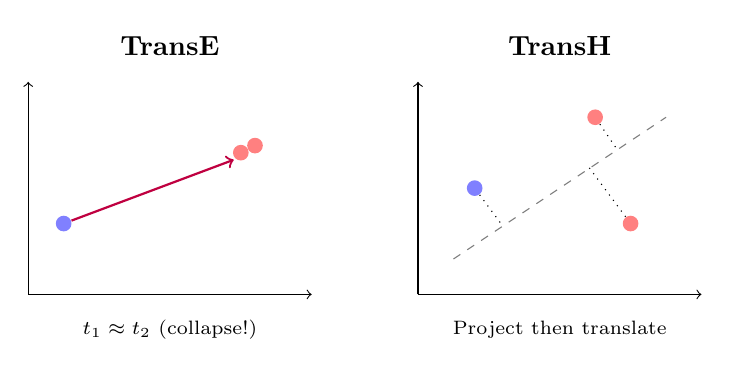
\begin{tikzpicture}[scale=0.9]
    % TransE
    \begin{scope}[xshift=0cm]
        \node[font=\bfseries] at (2, 3.5) {TransE};
        \draw[->] (0, 0) -- (4, 0);
        \draw[->] (0, 0) -- (0, 3);
        \node[circle, fill=blue!50, inner sep=2pt] (h1) at (0.5, 1) {};
        \node[circle, fill=red!50, inner sep=2pt] (t1a) at (3, 2) {};
        \node[circle, fill=red!50, inner sep=2pt] (t1b) at (3.2, 2.1) {};
        \draw[->, thick, purple] (h1) -- (2.9, 1.9);
        \node[font=\scriptsize] at (2, -0.5) {$t_1 \approx t_2$ (collapse!)};
    \end{scope}
    
    % TransH
    \begin{scope}[xshift=5.5cm]
        \node[font=\bfseries] at (2, 3.5) {TransH};
        \draw[->] (0, 0) -- (4, 0);
        \draw[->] (0, 0) -- (0, 3);
        % Hyperplane
        \draw[dashed, gray] (0.5, 0.5) -- (3.5, 2.5);
        \node[circle, fill=blue!50, inner sep=2pt] (h2) at (0.8, 1.5) {};
        \node[circle, fill=red!50, inner sep=2pt] (t2a) at (3, 1) {};
        \node[circle, fill=red!50, inner sep=2pt] (t2b) at (2.5, 2.5) {};
        % Projections
        \draw[dotted] (h2) -- (1.17, 1);
        \draw[dotted] (t2a) -- (2.4, 1.81);
        \draw[dotted] (t2b) -- (2.80, 2.06);
        \node[font=\scriptsize] at (2, -0.5) {Project then translate};
    \end{scope}
\end{tikzpicture}
\caption{TransE collapses multiple tails; TransH projects onto a hyperplane to allow separation.}
\label{shallow-embeddings:fig:transX}
\end{figure}


\subsubsection{Complex-Valued Embeddings: ComplEx and RotatE}

To model asymmetric relations with only $O(d)$ parameters per relation, we can use \textbf{complex numbers}.

\begin{definition}[ComplEx: Complex Embeddings]
Embed entities and relations in $\mathbb{C}^d$ (complex vector space). The scoring function uses a Hermitian inner product:
\begin{equation}
f_{\text{ComplEx}}(h, \tau, t) = \text{Re}\left(\langle \vect{z}_h, \vect{r}_\tau, \bar{\vect{z}}_t \rangle\right) = \text{Re}\left(\sum_{i=1}^{d} z_{h,i} \cdot r_{\tau,i} \cdot \bar{z}_{t,i}\right)
\end{equation}
where $\bar{\vect{z}}_t$ denotes the complex conjugate of $\vect{z}_t$, and $\text{Re}(\cdot)$ extracts the real part.
\end{definition}

\begin{mathbox}
\textbf{Why Complex Numbers Enable Asymmetry}

In $\mathbb{C}$, let $z = a + bi$ where $a, b \in \R$. The conjugate is $\bar{z} = a - bi$.

For two complex numbers $z_1 = a_1 + b_1 i$ and $z_2 = a_2 + b_2 i$:
\[
z_1 \cdot \bar{z}_2 = (a_1 + b_1 i)(a_2 - b_2 i) = (a_1 a_2 + b_1 b_2) + (b_1 a_2 - a_1 b_2)i
\]

If we swap $z_1$ and $z_2$:
\[
z_2 \cdot \bar{z}_1 = (a_1 a_2 + b_1 b_2) + (a_1 b_2 - b_1 a_2)i
\]

The \textbf{real parts are equal}, but the \textbf{imaginary parts differ by a sign}!

In ComplEx, using the relation embedding $r_\tau$ (also complex), we get:
\[
\text{Re}(z_h \cdot r_\tau \cdot \bar{z}_t) \neq \text{Re}(z_t \cdot r_\tau \cdot \bar{z}_h) \quad \text{in general}
\]

This asymmetry comes ``for free'' from the conjugate, without needing extra parameters!
\end{mathbox}

\begin{proposition}[ComplEx Asymmetry]
For ComplEx with embeddings $\vect{z}_h, \vect{z}_t, \vect{r}_\tau \in \mathbb{C}^d$:
\begin{equation}
f_{\text{ComplEx}}(h, \tau, t) - f_{\text{ComplEx}}(t, \tau, h) = 2 \sum_{i=1}^{d} \text{Re}(r_{\tau,i}) \cdot \text{Im}(z_{h,i}) \cdot \text{Im}(z_{t,i}) \cdot (-2)
\end{equation}
This is generally non-zero, enabling asymmetric relations.
\end{proposition}

\begin{example}
Let $d = 1$ with:
\[
z_h = 1 + 2i, \quad z_t = 2 + i, \quad r_\tau = 1 + 0.5i
\]

\textbf{Forward}: $(h, \tau, t)$
\begin{align*}
z_h \cdot r_\tau \cdot \bar{z}_t &= (1 + 2i)(1 + 0.5i)(2 - i) \\
&= (1 + 0.5i + 2i + i^2)(2 - i) \\
&= (0 + 2.5i)(2 - i) \\
&= 2.5i \cdot 2 - 2.5i \cdot i = 5i + 2.5 \\
f_{\text{ComplEx}}(h, \tau, t) &= \text{Re}(2.5 + 5i) = 2.5
\end{align*}

\textbf{Backward}: $(t, \tau, h)$
\begin{align*}
z_t \cdot r_\tau \cdot \bar{z}_h &= (2 + i)(1 + 0.5i)(1 - 2i) \\
&= (2 + i + i^2 + 0.5i)(1 - 2i) \\
&= (1 + 2i)(1 - 2i) \\
&= 1 - 4i^2 = 1 + 4 = 5 \\
f_{\text{ComplEx}}(t, \tau, h) &= \text{Re}(5) = 5
\end{align*}

We have $f(h, \tau, t) = 2.5 \neq 5 = f(t, \tau, h)$---asymmetry achieved!
\end{example}

\begin{definition}[RotatE: Rotation-Based Embedding]
Represent relations as \textbf{rotations} in complex space. Each component of the relation embedding has unit modulus: $|r_{\tau,i}| = 1$, so $r_{\tau,i} = e^{i\theta_{\tau,i}}$.

The scoring function is:
\begin{equation}
f_{\text{RotatE}}(h, \tau, t) = -\|\vect{z}_h \circ \vect{r}_\tau - \vect{z}_t\|
\end{equation}
where $\circ$ denotes element-wise (Hadamard) product.

\textbf{Intuition}: Each dimension of the head embedding is \emph{rotated} by angle $\theta_{\tau,i}$ to match the tail.
\end{definition}

\begin{figure}[htbp]
\centering
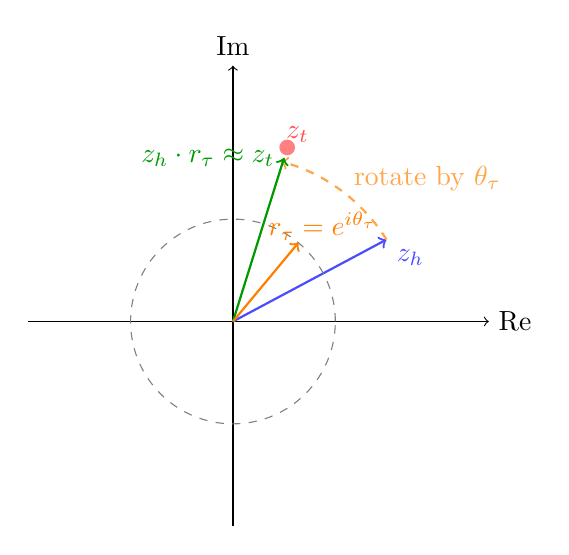
\begin{tikzpicture}[scale=1.3]
    % Complex plane
    \draw[->] (-2, 0) -- (2.5, 0) node[right] {Re};
    \draw[->] (0, -2) -- (0, 2.5) node[above] {Im};
    
    % Head embedding (one dimension)
    \draw[->, thick, blue!70] (0,0) -- (1.5, 0.8) node[below right] {$z_h$};
    
    % Rotation
    \draw[->, thick, orange!70, dashed] (1.5, 0.8) arc[start angle=32, end angle=75, radius=1.75];
    \node[orange!70] at (1.9, 1.4) {rotate by $\theta_\tau$};
    
    % Rotated = tail (approximately)
    \draw[->, thick, green!60!black] (0,0) -- (0.5, 1.6);
    \node[left, green!60!black] at (0.5, 1.6) {$z_h \cdot r_\tau \approx z_t$};
    
    % Tail embedding
    \node[circle, fill=red!50, inner sep=2pt] at (0.53, 1.7) {};
    \node[above, red!70] at (0.63, 1.65) {$z_t$};
    
    % Unit circle for r_tau
    \draw[gray, dashed] (0,0) circle[radius=1];
    \draw[->, thick, orange] (0,0) -- (0.64, 0.77);
    \node[right, orange] at (0.25, 0.93) {$r_\tau = e^{i\theta_\tau}$};
\end{tikzpicture}
\caption{RotatE: The relation rotates the head embedding toward the tail embedding in the complex plane.}
\label{shallow-embeddings:fig:rotate}
\end{figure}

\begin{proposition}[RotatE and Relation Patterns]
RotatE can model:
\begin{enumerate}
    \item \textbf{Symmetric relations}: Set $\theta_\tau = 0$ or $\theta_\tau = \pi$ (rotation by 0 or 180 degrees)
    \item \textbf{Antisymmetric relations}: Any $\theta_\tau \neq 0, \pi$
    \item \textbf{Inverse relations}: If $\tau_1$ is inverse of $\tau_2$, then $\theta_{\tau_1} = -\theta_{\tau_2}$
    \item \textbf{Composition}: If $\tau_3 = \tau_1 \circ \tau_2$, then $\theta_{\tau_3} = \theta_{\tau_1} + \theta_{\tau_2}$
\end{enumerate}
\end{proposition}

\begin{proof}[Proof of Composition]
For RotatE:
\begin{align*}
\vect{z}_h \circ \vect{r}_{\tau_1} &\approx \vect{z}_y \quad \text{(first hop)} \\
\vect{z}_y \circ \vect{r}_{\tau_2} &\approx \vect{z}_t \quad \text{(second hop)}
\end{align*}
Substituting:
\[
(\vect{z}_h \circ \vect{r}_{\tau_1}) \circ \vect{r}_{\tau_2} = \vect{z}_h \circ (\vect{r}_{\tau_1} \circ \vect{r}_{\tau_2}) \approx \vect{z}_t
\]
Since $r_{\tau_1,i} \cdot r_{\tau_2,i} = e^{i\theta_{\tau_1,i}} \cdot e^{i\theta_{\tau_2,i}} = e^{i(\theta_{\tau_1,i} + \theta_{\tau_2,i})}$, we have $\vect{r}_{\tau_3} = \vect{r}_{\tau_1} \circ \vect{r}_{\tau_2}$. $\blacksquare$
\end{proof}

\subsection{Comparison of Multi-Relational Decoders}

\begin{table}[htbp]
\centering
\caption{Comparison of Multi-Relational Decoders}
\begin{tabular}{@{}lcccccc@{}}
\toprule
\textbf{Model} & \textbf{Scoring Function} & \textbf{Params/Rel} & \textbf{Symm.} & \textbf{Antisymm.} & \textbf{Inverse} & \textbf{Compos.} \\
\midrule
RESCAL & $\vect{z}_h^\top \vect{R}_\tau \vect{z}_t$ & $O(d^2)$ & \checkmark & \checkmark & \checkmark & \checkmark \\
DistMult & $\langle \vect{z}_h, \vect{r}_\tau, \vect{z}_t \rangle$ & $O(d)$ & \checkmark & $\times$ & $\times$ & $\times$ \\
TransE & $-\|\vect{z}_h + \vect{r}_\tau - \vect{z}_t\|$ & $O(d)$ & $\times$ & \checkmark & \checkmark & \checkmark \\
TransH & proj. + translation & $O(d)$ & \checkmark & \checkmark & $\times$ & $\times$ \\
ComplEx & $\text{Re}(\langle \vect{z}_h, \vect{r}_\tau, \bar{\vect{z}}_t \rangle)$ & $O(d)$ & \checkmark & \checkmark & \checkmark & $\times$ \\
RotatE & $-\|\vect{z}_h \circ \vect{r}_\tau - \vect{z}_t\|$ & $O(d)$ & \checkmark & \checkmark & \checkmark & \checkmark \\
\bottomrule
\end{tabular}
\label{shallow-embeddings:tab:kg_comparison}
\end{table}

\begin{keyinsight}
\textbf{Choosing a Decoder}:
\begin{itemize}
    \item \textbf{Few relations, lots of data}: RESCAL (most expressive)
    \item \textbf{Mostly symmetric relations}: DistMult (simplest, efficient)
    \item \textbf{Strong compositional patterns}: TransE or RotatE
    \item \textbf{Mixed symmetric/asymmetric}: ComplEx or RotatE
    \item \textbf{General recommendation}: RotatE is often a good default---it's efficient ($O(d)$ per relation) yet captures all common relation patterns
\end{itemize}
\end{keyinsight}

\subsection{A Running Example: Small Knowledge Graph}

Let's trace through embedding a small knowledge graph with $d = 2$ dimensions.

\begin{example}[Complete Walkthrough]
Consider the knowledge graph:
\begin{center}
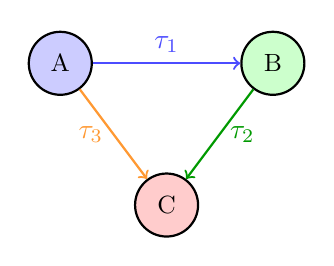
\begin{tikzpicture}[
    entity/.style={circle, draw, thick, minimum size=0.8cm, font=\small},
    scale=0.9
]
    \node[entity, fill=blue!20] (A) at (0, 0) {A};
    \node[entity, fill=green!20] (B) at (3, 0) {B};
    \node[entity, fill=red!20] (C) at (1.5, -2) {C};
    
    \draw[->, thick, blue!70] (A) -- node[above] {$\tau_1$} (B);
    \draw[->, thick, green!60!black] (B) -- node[right] {$\tau_2$} (C);
    \draw[->, thick, orange!80] (A) -- node[left] {$\tau_3$} (C);
\end{tikzpicture}
\end{center}

Triples: $\{(A, \tau_1, B), (B, \tau_2, C), (A, \tau_3, C)\}$

Note: We expect $\tau_3$ to be the composition of $\tau_1$ and $\tau_2$.

\textbf{Step 1: Initialize} (random)
\begin{align*}
\vect{z}_A &= (1.0, 0.5), \quad \vect{z}_B = (0.3, 0.8), \quad \vect{z}_C = (-0.2, 0.9) \\
\vect{r}_{\tau_1} &= (0.5, 0.2), \quad \vect{r}_{\tau_2} = (-0.3, 0.1), \quad \vect{r}_{\tau_3} = (0.1, 0.4)
\end{align*}

\textbf{Step 2: Compute TransE scores for positive triples}
\begin{align*}
f(A, \tau_1, B) &= -\|(1.0, 0.5) + (0.5, 0.2) - (0.3, 0.8)\|_2 \\
&= -\|(1.2, -0.1)\|_2 = -\sqrt{1.44 + 0.01} = -1.20
\end{align*}
(This is a poor score---the translation doesn't match well.)

\textbf{Step 3: Gradient update for $(A, \tau_1, B)$}

Let $\vect{e} = \vect{z}_A + \vect{r}_{\tau_1} - \vect{z}_B = (1.2, -0.1)$.

Gradients (for $L_2$ norm):
\begin{align*}
\nabla_{\vect{z}_A} \|\vect{e}\|_2 &= \vect{e}/\|\vect{e}\| = (0.996, -0.083) \\
\nabla_{\vect{r}_{\tau_1}} \|\vect{e}\|_2 &= \vect{e}/\|\vect{e}\| = (0.996, -0.083) \\
\nabla_{\vect{z}_B} \|\vect{e}\|_2 &= -\vect{e}/\|\vect{e}\| = (-0.996, 0.083)
\end{align*}

With learning rate $\eta = 0.1$, updates push $\vect{z}_A + \vect{r}_{\tau_1}$ closer to $\vect{z}_B$.

\textbf{After training} (converged embeddings):
\begin{align*}
\vect{z}_A &\approx (0.0, 0.0), \quad \vect{z}_B \approx (1.0, 0.0), \quad \vect{z}_C \approx (1.0, 1.0) \\
\vect{r}_{\tau_1} &\approx (1.0, 0.0), \quad \vect{r}_{\tau_2} \approx (0.0, 1.0), \quad \vect{r}_{\tau_3} \approx (1.0, 1.0)
\end{align*}

\textbf{Verify compositionality}: $\vect{r}_{\tau_3} = (1.0, 1.0) = (1.0, 0.0) + (0.0, 1.0) = \vect{r}_{\tau_1} + \vect{r}_{\tau_2}$ \checkmark

\textbf{Link prediction}: Does $(A, \tau_2, C)$ hold?
\[
f(A, \tau_2, C) = -\|(0, 0) + (0, 1) - (1, 1)\| = -\|(-1, 0)\| = -1.0
\]
Score is poor ($-1.0$), so model predicts this triple is unlikely---correct!
\end{example}

\subsection{Practical Considerations}

\begin{remark}[Training Strategies]
\leavevmode
\begin{enumerate}
    \item \textbf{Mini-batch training}: Sample triples, generate negatives, compute loss
    \item \textbf{Entity/relation normalization}: Often helpful to constrain $\|\vect{z}_v\| = 1$ or $\|\vect{r}_\tau\| = 1$
    \item \textbf{Self-adversarial negative sampling}: Weight negatives by their current score (harder negatives count more)
    \item \textbf{Type constraints}: Use entity types to filter invalid negatives
\end{enumerate}
\end{remark}

\begin{remark}[Evaluation Protocols]
\leavevmode
Standard metrics for knowledge graph completion:
\begin{itemize}
    \item \textbf{Mean Rank (MR)}: Average rank of true triples among all candidates
    \item \textbf{Mean Reciprocal Rank (MRR)}: Average of $1/\text{rank}$
    \item \textbf{Hits@$k$}: Fraction of true triples ranked in top $k$
\end{itemize}
Always use the \textbf{filtered} setting: remove other true triples from the candidate set.
\end{remark}

\begin{remark}[Limitations and Future Directions]
Shallow knowledge graph embeddings have limitations similar to simple graph embeddings:
\begin{itemize}
    \item Cannot generalize to unseen entities (transductive)
    \item Don't leverage entity features or descriptions
    \item Limited reasoning capabilities (e.g., negation, counting)
\end{itemize}
\textbf{Graph Neural Networks} for multi-relational data (R-GCN, CompGCN) address some of these issues---see the next major topic on deep graph learning.
\end{remark}


% ============================================================================
% SECTION 6: EDGE AND GRAPH EMBEDDINGS
% ============================================================================
\section{Beyond Nodes: Edge and Graph Embeddings}

\subsection{Edge2Vec: Embedding Edges}

Once we have node embeddings, we can create edge embeddings by combining endpoint embeddings.

\begin{definition}[Edge Embedding Operators]
For edge $(i, j)$ with node embeddings $\vect{y}_i, \vect{y}_j$:
\begin{align*}
\text{Average}: & \quad \vect{e}_{ij} = \frac{\vect{y}_i + \vect{y}_j}{2} \\
\text{Hadamard}: & \quad \vect{e}_{ij} = \vect{y}_i \odot \vect{y}_j \quad \text{(element-wise product)} \\
\text{L1 distance}: & \quad \vect{e}_{ij} = |\vect{y}_i - \vect{y}_j| \\
\text{L2 distance}: & \quad \vect{e}_{ij} = (\vect{y}_i - \vect{y}_j)^2
\end{align*}
\end{definition}

\begin{example}
Suppose $\vect{y}_2 = (0.8, 0.3)$ and $\vect{y}_4 = (0.2, 0.7)$ for the bridge edge (2,4):

\begin{align*}
\text{Average}: & \quad \vect{e}_{24} = (0.5, 0.5) \\
\text{Hadamard}: & \quad \vect{e}_{24} = (0.16, 0.21) \\
\text{L1}: & \quad \vect{e}_{24} = (0.6, 0.4)
\end{align*}

\textbf{Interpretation}:
\begin{itemize}
    \item \textbf{Average}: The edge embedding is ``between'' the two nodes---good for interpolation
    \item \textbf{Hadamard}: Captures shared structure (both dimensions somewhat active)
    \item \textbf{L1}: Captures how different the nodes are---useful for predicting edge types
\end{itemize}
\end{example}

\textbf{Use case}: Link prediction! Given an edge embedding, train a classifier to predict if the edge exists.

\subsection{Graph2Vec: Embedding Entire Graphs}

\begin{whybox}
Sometimes we want to compare entire graphs, not just nodes:
\begin{itemize}
    \item Is this molecule similar to that molecule?
    \item Is this social network similar to that one?
    \item Classify graphs by type (toxic vs. non-toxic compounds)
\end{itemize}
\end{whybox}

\begin{definition}[Graph2Vec]
Idea: Treat a graph as a ``document'' and its subgraph patterns as ``words.''
\begin{enumerate}
    \item Extract rooted subgraph patterns around each node (using Weisfeiler-Lehman hashing)
    \item Each graph becomes a ``bag of subgraphs''
    \item Use Doc2Vec to learn graph embeddings
\end{enumerate}
\end{definition}

\begin{figure}[htbp]
\centering
\begin{tikzpicture}[
    main/.style={circle, draw, thick, minimum size=0.5cm, font=\tiny},
    subgraph/.style={rectangle, draw, rounded corners, minimum width=2cm, minimum height=1.5cm}
]
    % Original graph
    \node[font=\bfseries] at (0, 2) {Graph $G$};
    \node[main] (a) at (-0.5, 0.5) {1};
    \node[main] (b) at (0.5, 0.5) {2};
    \node[main] (c) at (0, -0.5) {3};
    \draw (a) -- (b) -- (c) -- (a);
    
    % Arrow
    \draw[-{Stealth}, thick] (1.2, 0) -- (2.3, 0) node[midway, above, font=\small] {WL};
    
    % Subgraphs
    \node[font=\bfseries] at (4.5, 2) {Subgraph ``words''};
    
    \begin{scope}[xshift=3.5cm, yshift=0.3cm, scale=0.6]
        \node[main, fill=yellow!50] (s1) at (0,0) {};
        \node[main] (s2) at (0.7, 0) {};
        \node[main] (s3) at (0.35, -0.6) {};
        \draw (s1) -- (s2);
        \draw (s1) -- (s3);
        \node[below of=s3, yshift=0.7cm, font=\tiny] {$h_1$: degree-2};
    \end{scope}
    
    \begin{scope}[xshift=5.5cm, yshift=0.3cm, scale=0.6]
        \node[main, fill=yellow!50] (t1) at (0,0) {};
        \node[main] (t2) at (0.7, 0) {};
        \node[main] (t3) at (0.35, -0.6) {};
        \draw (t1) -- (t2) -- (t3) -- (t1);
        \node[below of=t3, yshift=0.7cm, font=\tiny] {$h_2$: triangle};
    \end{scope}
    
    % Doc representation
    \draw[-{Stealth}, thick] (6.5, 0) -- (7.5, 0);
    \node[font=\small] at (9, 0) {$G \to \{h_1, h_1, h_1, h_2, \ldots\}$};
    \node[font=\small] at (9, -0.5) {(``document'')};
    
\end{tikzpicture}
\caption{Graph2Vec: extract subgraph patterns as ``words,'' represent graph as document, learn embedding.}
\label{shallow-embeddings:fig:graph2vec}
\end{figure}


% ============================================================================
% SECTION 7: SUMMARY AND COMPARISON
% ============================================================================
\section{Putting It All Together}

\subsection{Method Comparison}

\begin{table}[htbp]
\centering
\caption{Summary of Shallow Embedding Methods}
\begin{tabular}{@{}lccc@{}}
\toprule
\textbf{Method} & \textbf{Proximity Type} & \textbf{Best For} & \textbf{Directed?} \\
\midrule
GF & First-order & Simple, fast baseline & No \\
HOPE & High-order (Katz, etc.) & Directed graphs, asymmetry & Yes \\
GraRep & Multi-scale & Need both local \& global & Partial \\
\midrule
DeepWalk & Multi-hop (random walk) & General purpose & No \\
Node2Vec & Tunable local/global & When you need control & No \\
\midrule
\multicolumn{4}{c}{\textit{Multi-Relational / Knowledge Graph Methods}} \\
\midrule
RESCAL & Bilinear & Rich relations, small KG & Yes \\
DistMult & Diagonal bilinear & Symmetric relations & No \\
TransE & Translation & Compositional patterns & Yes \\
ComplEx & Complex bilinear & Mixed symmetry relations & Yes \\
RotatE & Rotation & General KG completion & Yes \\
\bottomrule
\end{tabular}
\end{table}

\subsection{Decision Flowchart}

\begin{figure}[htbp]
\centering
\begin{tikzpicture}[
    decision/.style={diamond, draw, thick, fill=yellow!20, text width=2.5cm, align=center, inner sep=1pt},
    block/.style={rectangle, draw, thick, fill=blue!20, text width=2.5cm, align=center, rounded corners, minimum height=1cm},
    arrow/.style={-{Stealth}, thick}
]
    \node[decision] (dir) {Directed graph?};
    \node[block, below left=1.5cm and 1cm of dir] (hope) {HOPE};
    \node[decision, below right=1.5cm and 1cm of dir] (scale) {Need multi-scale?};
    \node[block, below left=1.5cm and 0.5cm of scale] (grarep) {GraRep};
    \node[decision, below right=1.5cm and 0.5cm of scale] (control) {Need walk control?};
    \node[block, below left=1.2cm and 0.3cm of control] (n2v) {Node2Vec};
    \node[block, below right=1.2cm and 0.3cm of control] (dw) {DeepWalk};
    
    \draw[arrow] (dir) -- node[left, font=\small] {Yes} (hope);
    \draw[arrow] (dir) -- node[right, font=\small] {No} (scale);
    \draw[arrow] (scale) -- node[left, font=\small] {Yes} (grarep);
    \draw[arrow] (scale) -- node[right, font=\small] {No} (control);
    \draw[arrow] (control) -- node[left, font=\small] {Yes} (n2v);
    \draw[arrow] (control) -- node[right, font=\small] {No} (dw);
\end{tikzpicture}
\caption{Choosing an embedding method.}
\end{figure}

\subsection{Key Takeaways}

\begin{keyinsight}
\begin{enumerate}
    \item \textbf{All methods share a common goal}: Map nodes to vectors so that graph similarity becomes vector similarity.
    
    \item \textbf{Matrix factorization and skip-gram are deeply connected}: Skip-gram methods implicitly factorize a matrix related to random walk probabilities!
    
    \item \textbf{Different methods capture different structure}:
    \begin{itemize}
        \item First-order: direct connections (GF, LINE first-order)
        \item Second-order: shared neighbors (LINE second-order)
        \item High-order: paths, global structure (HOPE, DeepWalk, Node2Vec)
    \end{itemize}
    
    \item \textbf{Random walks are powerful}: They naturally sample paths of varying lengths, capturing multi-scale structure without explicit matrix computation.
    
    \item \textbf{The Laplacian family keeps appearing}: Whether in spectral embedding, random walks, or graph signal processing, these matrices encode fundamental graph structure.
\end{enumerate}
\end{keyinsight}

\subsection{What's Next?}

Shallow methods have a key limitation: they learn a fixed embedding for each node. This means:
\begin{itemize}
    \item No generalization to new nodes (must recompute everything)
    \item No use of node features (attributes like age, location)
    \item Limited expressive power for complex patterns
\end{itemize}

\textbf{Deep methods} (Graph Neural Networks) address these by learning a function that \emph{generates} embeddings from local neighborhood structure. But that's for the next chapter!


% ============================================================================
% BIBLIOGRAPHY
% ============================================================================
\begin{thebibliography}{99}

\bibitem{shallow-embeddings:perozzi2014}
B. Perozzi, R. Al-Rfou, and S. Skiena.
\newblock DeepWalk: Online learning of social representations.
\newblock In \emph{KDD}, 2014.

\bibitem{shallow-embeddings:grover2016}
A. Grover and J. Leskovec.
\newblock node2vec: Scalable feature learning for networks.
\newblock In \emph{KDD}, 2016.

\bibitem{shallow-embeddings:ou2016}
M. Ou, P. Cui, J. Pei, Z. Zhang, and W. Zhu.
\newblock Asymmetric transitivity preserving graph embedding.
\newblock In \emph{KDD}, 2016.

\bibitem{shallow-embeddings:cao2015}
S. Cao, W. Lu, and Q. Xu.
\newblock GraRep: Learning graph representations with global structural information.
\newblock In \emph{CIKM}, 2015.

\bibitem{shallow-embeddings:qiu2018}
J. Qiu, Y. Dong, H. Ma, J. Li, K. Wang, and J. Tang.
\newblock Network embedding as matrix factorization: Unifying DeepWalk, LINE, PTE, and node2vec.
\newblock In \emph{WSDM}, 2018.

\bibitem{shallow-embeddings:nickel2011}
M. Nickel, V. Tresp, and H.-P. Kriegel.
\newblock A three-way model for collective learning on multi-relational data.
\newblock In \emph{ICML}, 2011.

\bibitem{shallow-embeddings:bordes2013}
A. Bordes, N. Usunier, A. Garcia-Duran, J. Weston, and O. Yakhnenko.
\newblock Translating embeddings for modeling multi-relational data.
\newblock In \emph{NeurIPS}, 2013.

\bibitem{shallow-embeddings:yang2015}
B. Yang, W.-t. Yih, X. He, J. Gao, and L. Deng.
\newblock Embedding entities and relations for learning and inference in knowledge bases.
\newblock In \emph{ICLR}, 2015.

\bibitem{shallow-embeddings:trouillon2016}
T. Trouillon, J. Welbl, S. Riedel, E. Gaussier, and G. Bouchard.
\newblock Complex embeddings for simple link prediction.
\newblock In \emph{ICML}, 2016.

\bibitem{shallow-embeddings:sun2019}
Z. Sun, Z.-H. Deng, J.-Y. Nie, and J. Tang.
\newblock RotatE: Knowledge graph embedding by relational rotation in complex space.
\newblock In \emph{ICLR}, 2019.

\bibitem{shallow-embeddings:wang2014}
Z. Wang, J. Zhang, J. Feng, and Z. Chen.
\newblock Knowledge graph embedding by translating on hyperplanes.
\newblock In \emph{AAAI}, 2014.

\bibitem{shallow-embeddings:hamilton2020}
W.~L. Hamilton.
\newblock \emph{Graph Representation Learning}.
\newblock Morgan \& Claypool Publishers, 2020.

\end{thebibliography}
\end{notechapter}
